\section{Goals}
\begin{itemize}[label=$\bullet$, itemsep=-1pt, leftmargin=*]
	%    \setlength\itemsep{0.5em}
	% \item Students are able to create projects on an IDE
	% \item Students can demonstrate his/her knowledge of the structure of a C program
	% \item Students can demonstrate his/her knowledge of C data types
	% \item Students can demonstrate his/her knowledge of C operators
	% \item Students are able to use function to read inputs from keyboard
	% \item Students are able to use function to print texts on screen
	\item Students can create projects within the IDE.
	\item Students can demonstrate their knowledge about program structure in the C language
	\item Students can demonstrate their knowledge about data types in the C language
	\item Students can demonstrate their knowledge of data types in the C language
	\item Students are able to use functions to read input from the keyboard
	\item Students are able to use functions to print text on the screen

\end{itemize}
\section{Introduction to C Programming Language}

The C language was developed by Dennis M. Ritchie and Brian W. Kernighan in the early 1970s.\\
There are several standards for the C programming language. There are several guidelines for writing C programming language. Below are some of the standards:
\begin{enumerate}
	\item Kernighan \& Ritchie Definition(K\&R)
	\item ANSI-C (X-3.159 -1989-)
	\item AT\&T (for superset C, C++) definition, and
	\item GNU Coding Standards
\end{enumerate}
\subsection*{}Implementation and uses of the C programming language
\begin{enumerate}
	\item Creating operating systems and it's system programs
	\item Programmin language that is "very close" to hardware (e.g., for device control).
	\item Developing toolkits
	\item Writing programs
\end{enumerate}
\section{IDE (Integrated Development Environment)}
IDE stands for "Integrated Development Environment" in English. In Bahasa Indonesia, IDE can be translated as "Lingkungan Pengembangan Terintegrasi" or "Ruang Kerja Pengembangan Terpadu." IDE is a software designed to assist software developers in the process of development, coding, and testing computer applications.
\\
Here are several list of C programming language IDE applications that can be used.
\begin{itemize}
	\item Code::Blocks
\end{itemize}
\section{Creating new project in IDE Code::Blocks}
\subsection{Steps to create a new project}
\begin{enumerate}
	\item Go to File $>$ New $>$ Project
	      \begin{figure}[H]
		      \centering
		      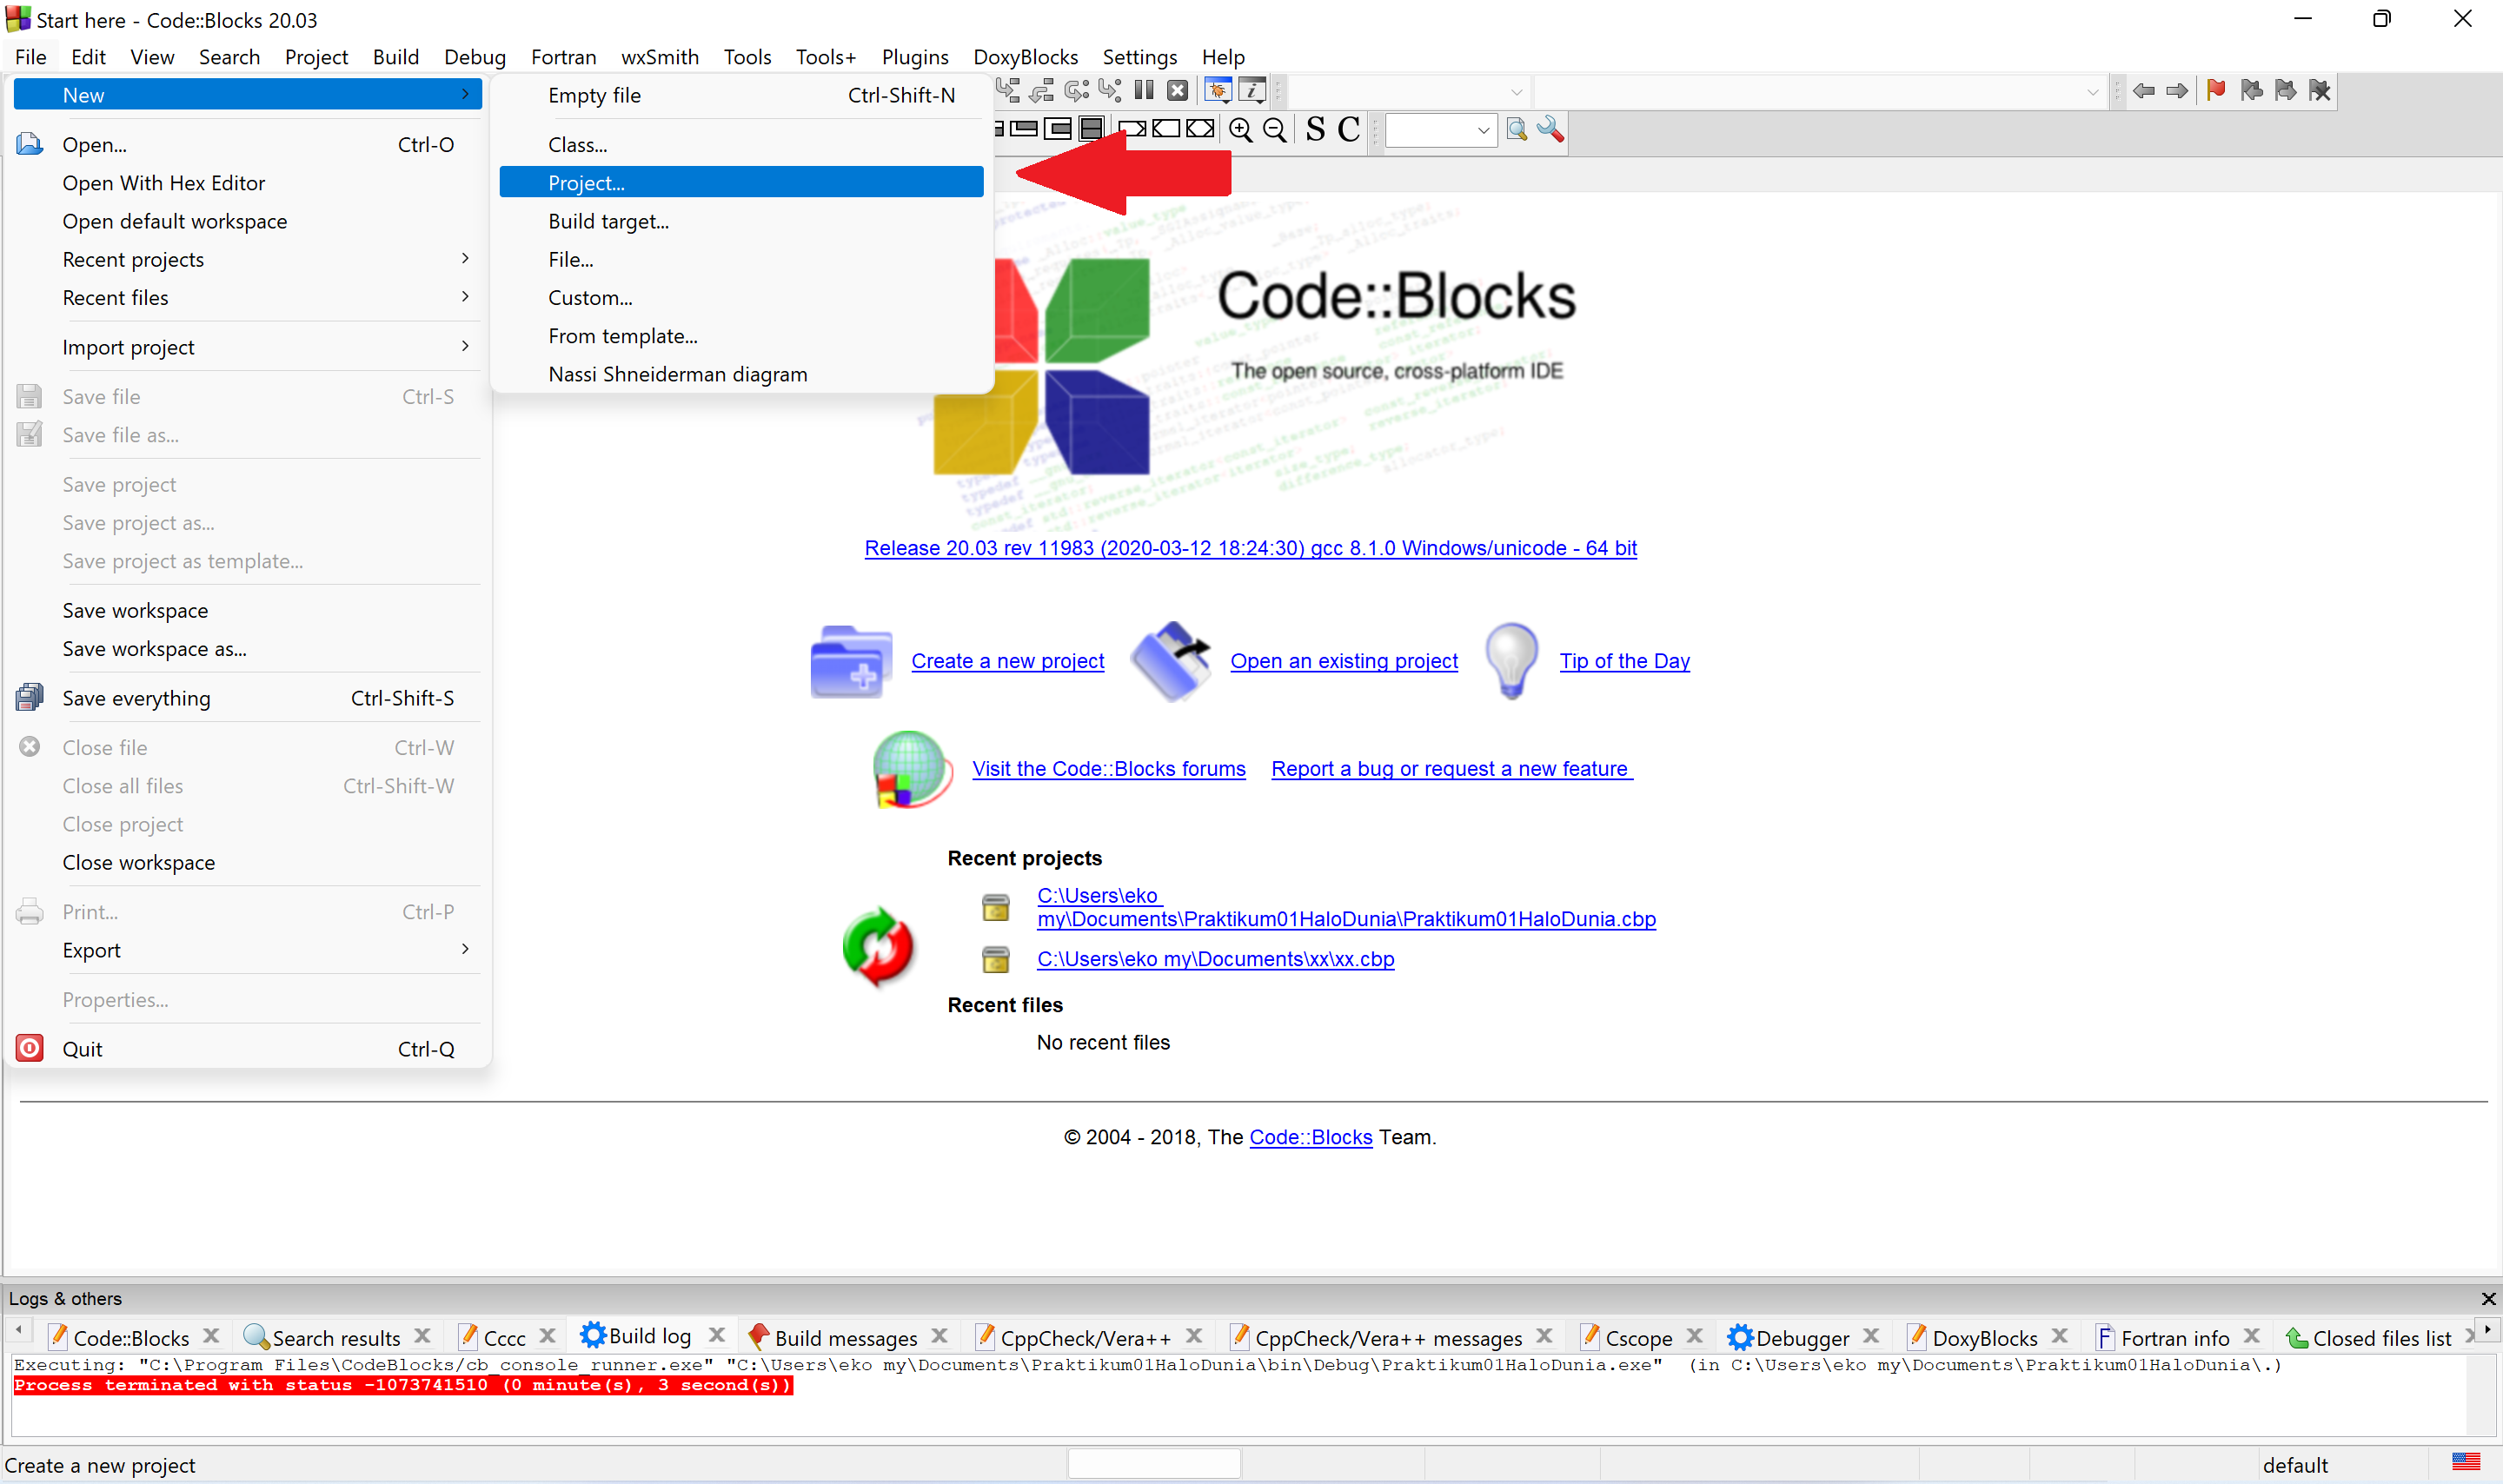
\includegraphics[width=0.7\linewidth]{P1/img/screenshot002.png}
		      \caption{}
		      \label{fig:screenshot002}
	      \end{figure}
	\item Click on Console Application
	      \begin{figure}[H]
		      \centering
		      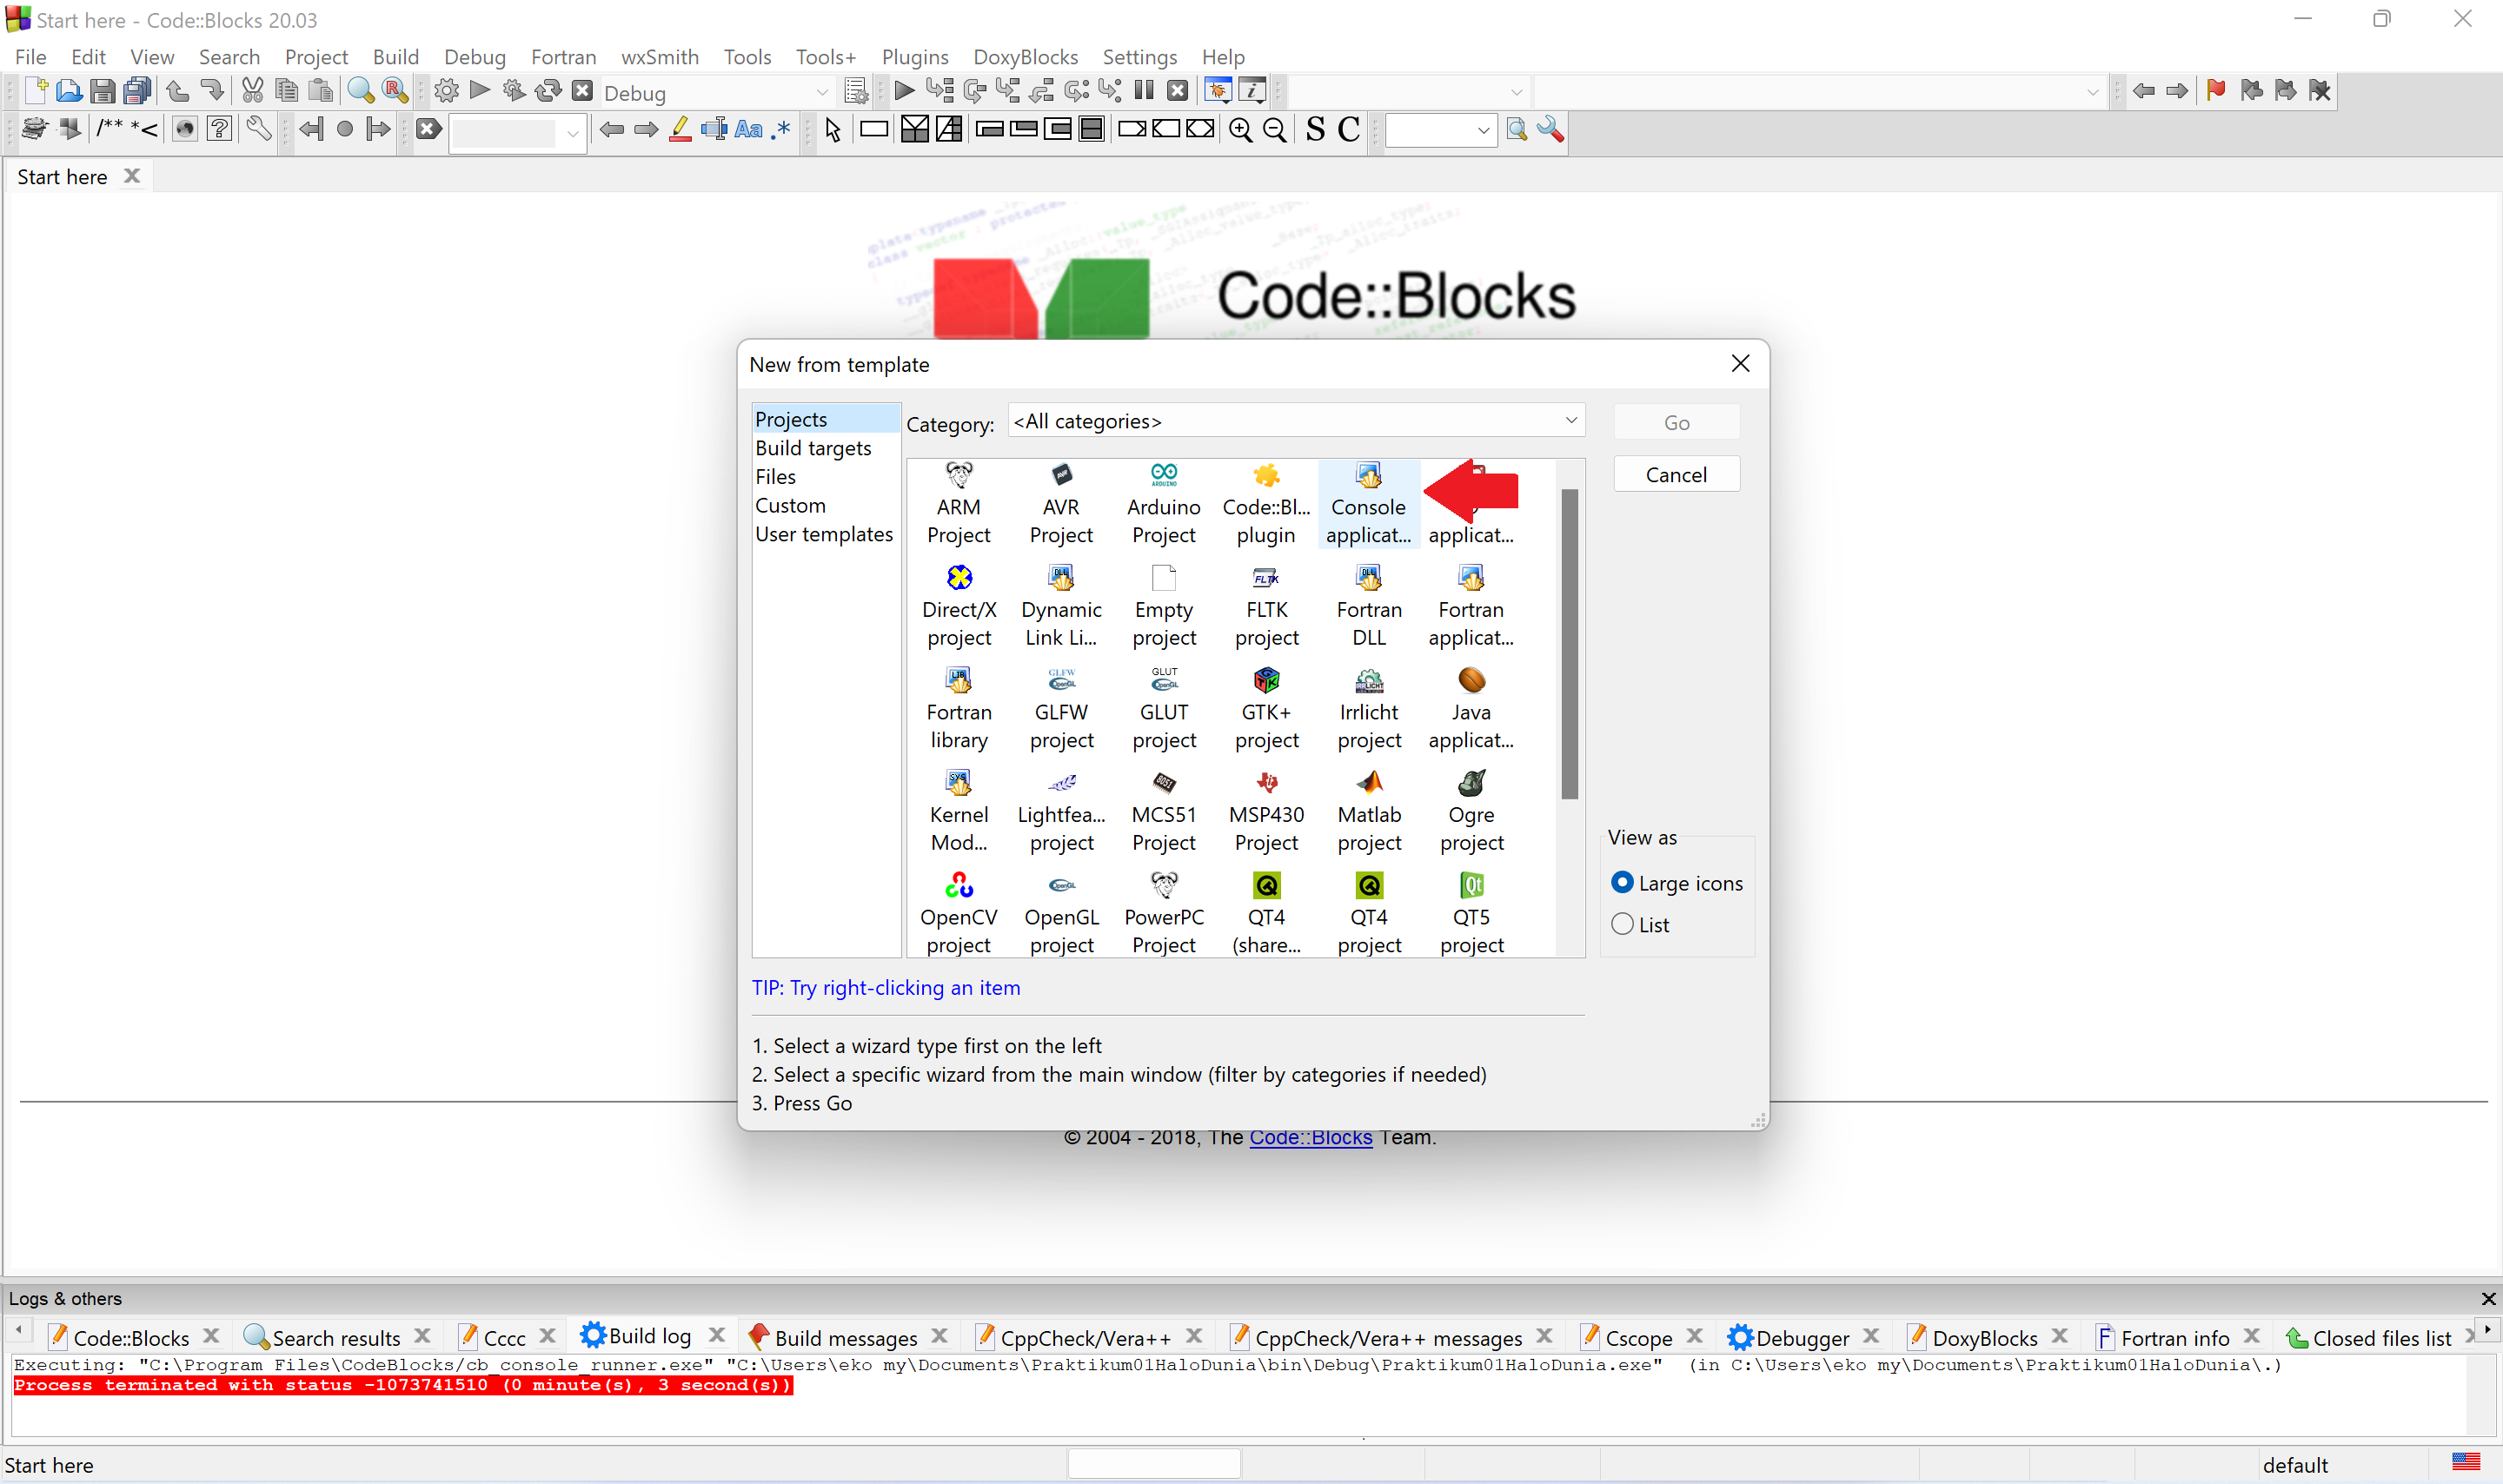
\includegraphics[width=0.7\linewidth]{P1/img/screenshot004.png}
		      \caption{}
		      \label{fig:screenshot004}
	      \end{figure}
	\item Choose C as the programming language
	      \begin{figure}[H]
		      \centering
		      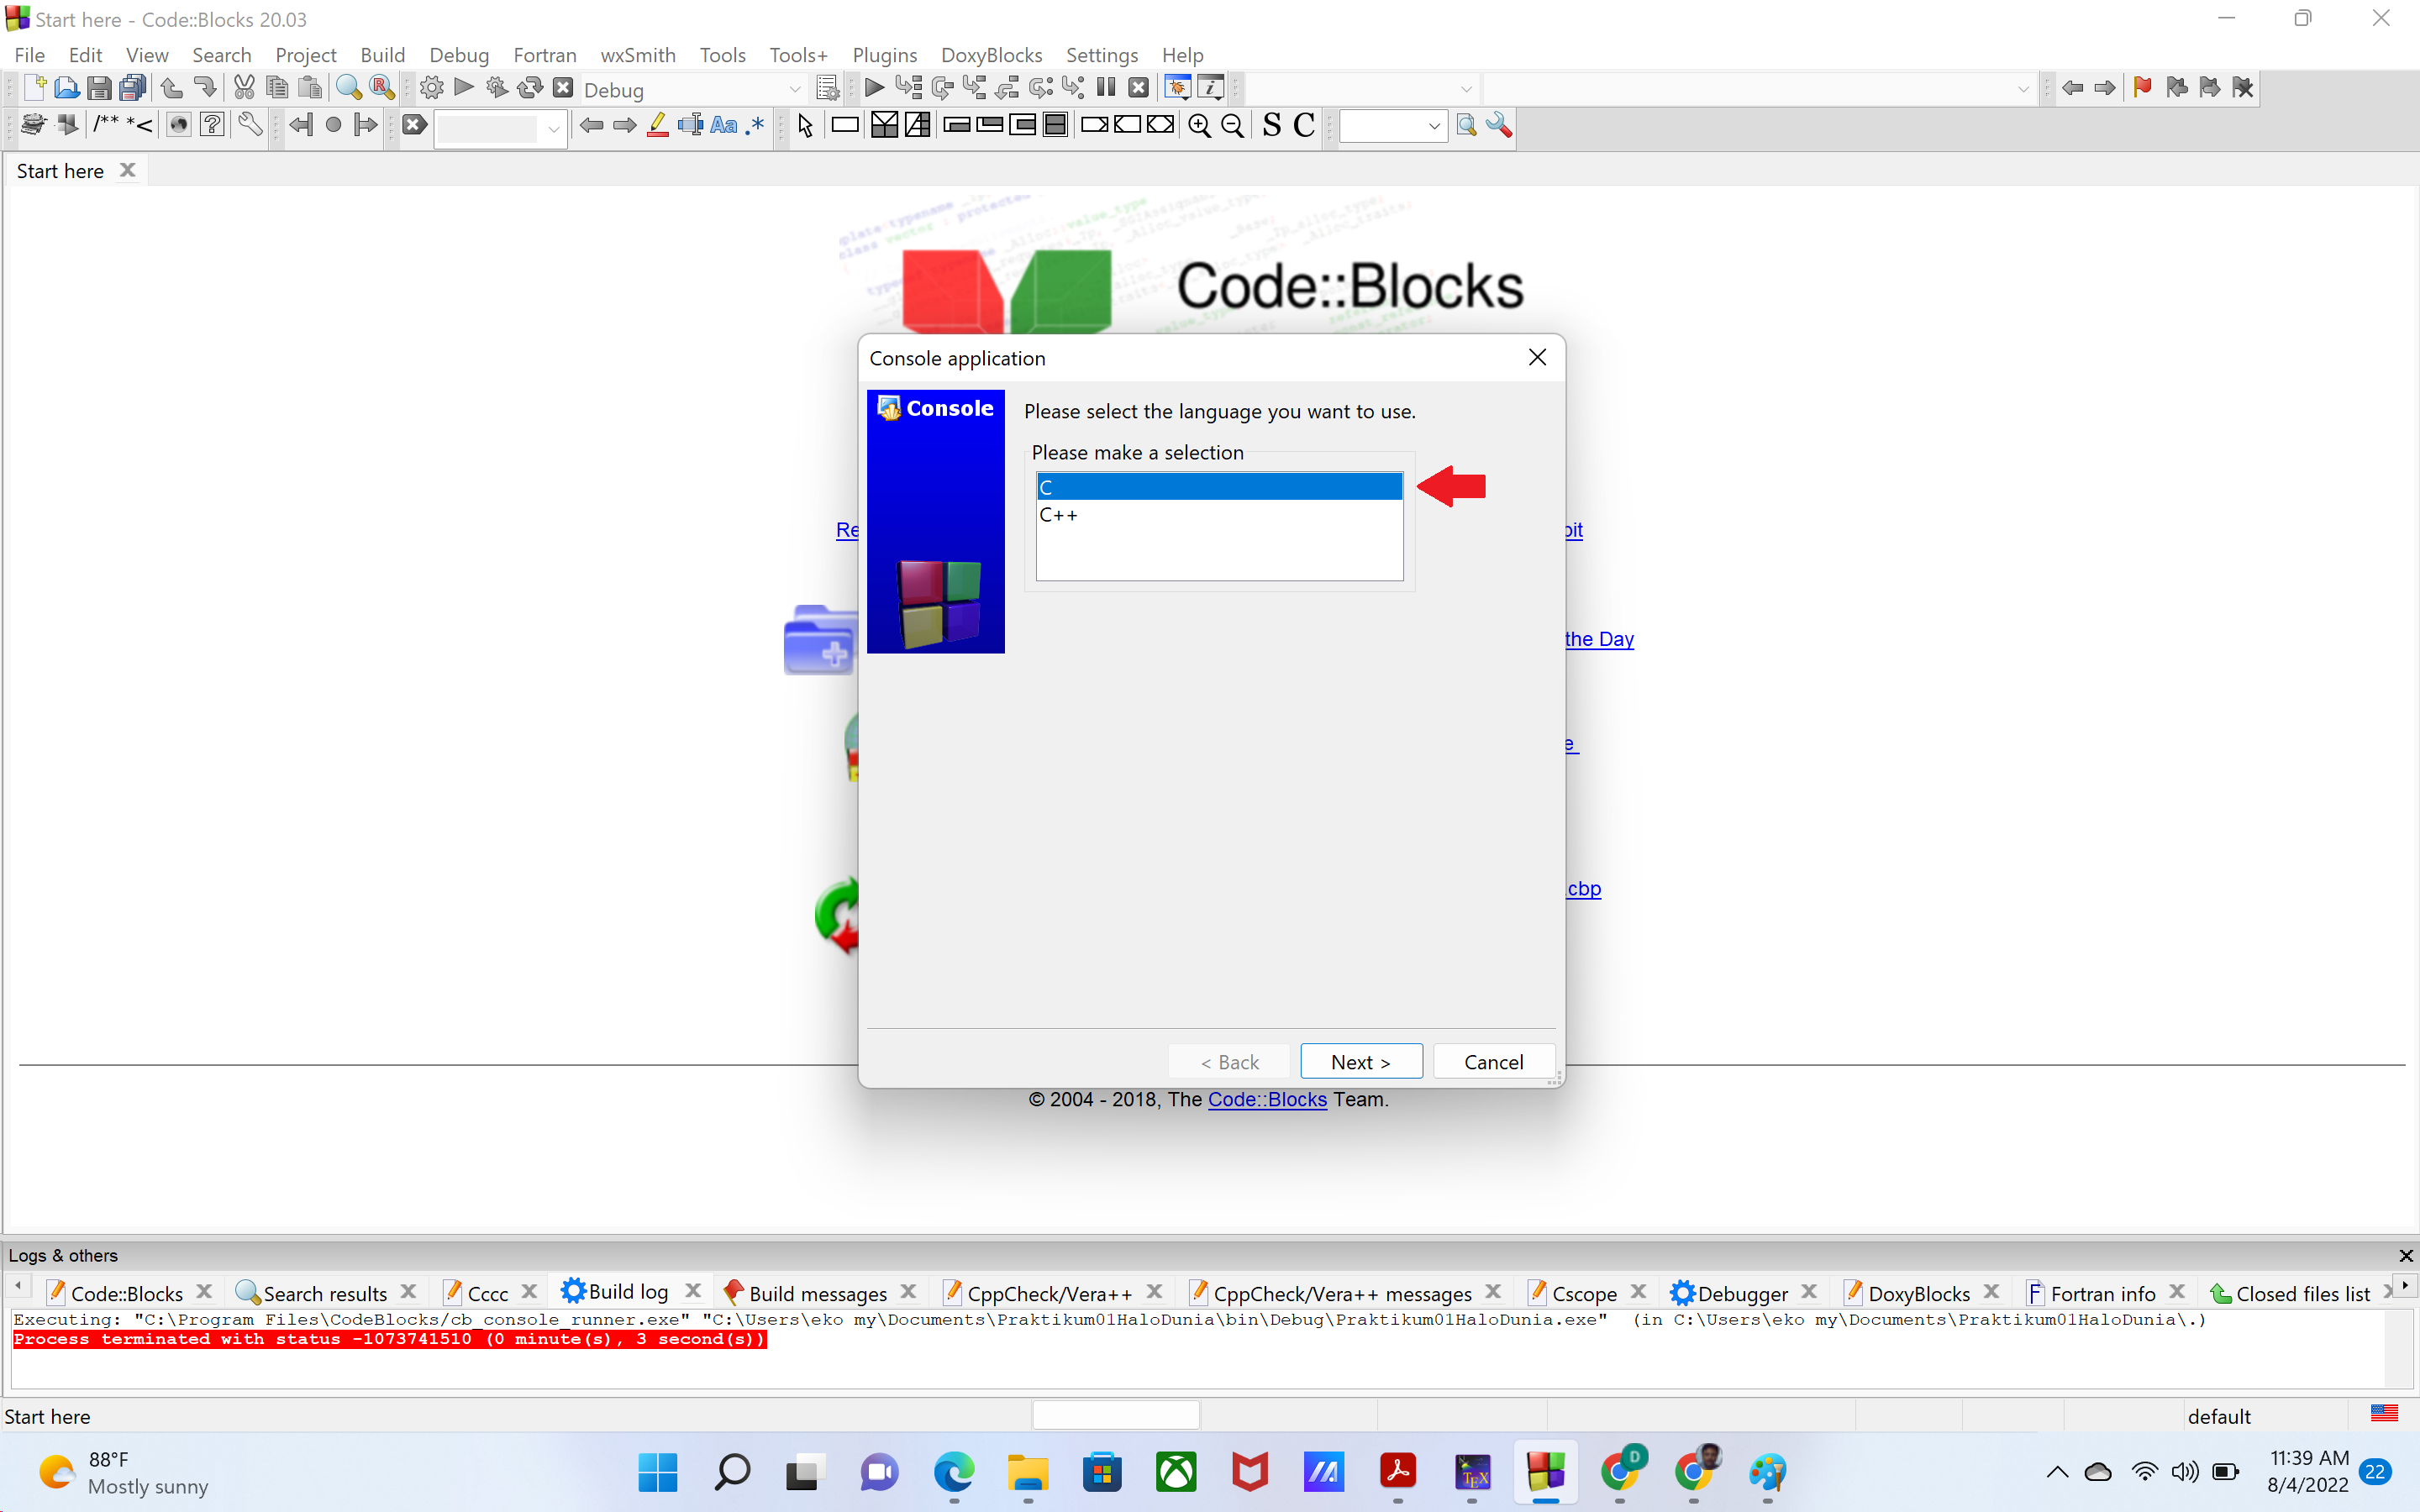
\includegraphics[width=0.7\linewidth]{P1/img/screenshot005.png}
		      \caption{}
		      \label{fig:screenshot005}
	      \end{figure}
	\item Insert your project name
	      \begin{figure}[H]
		      \centering
		      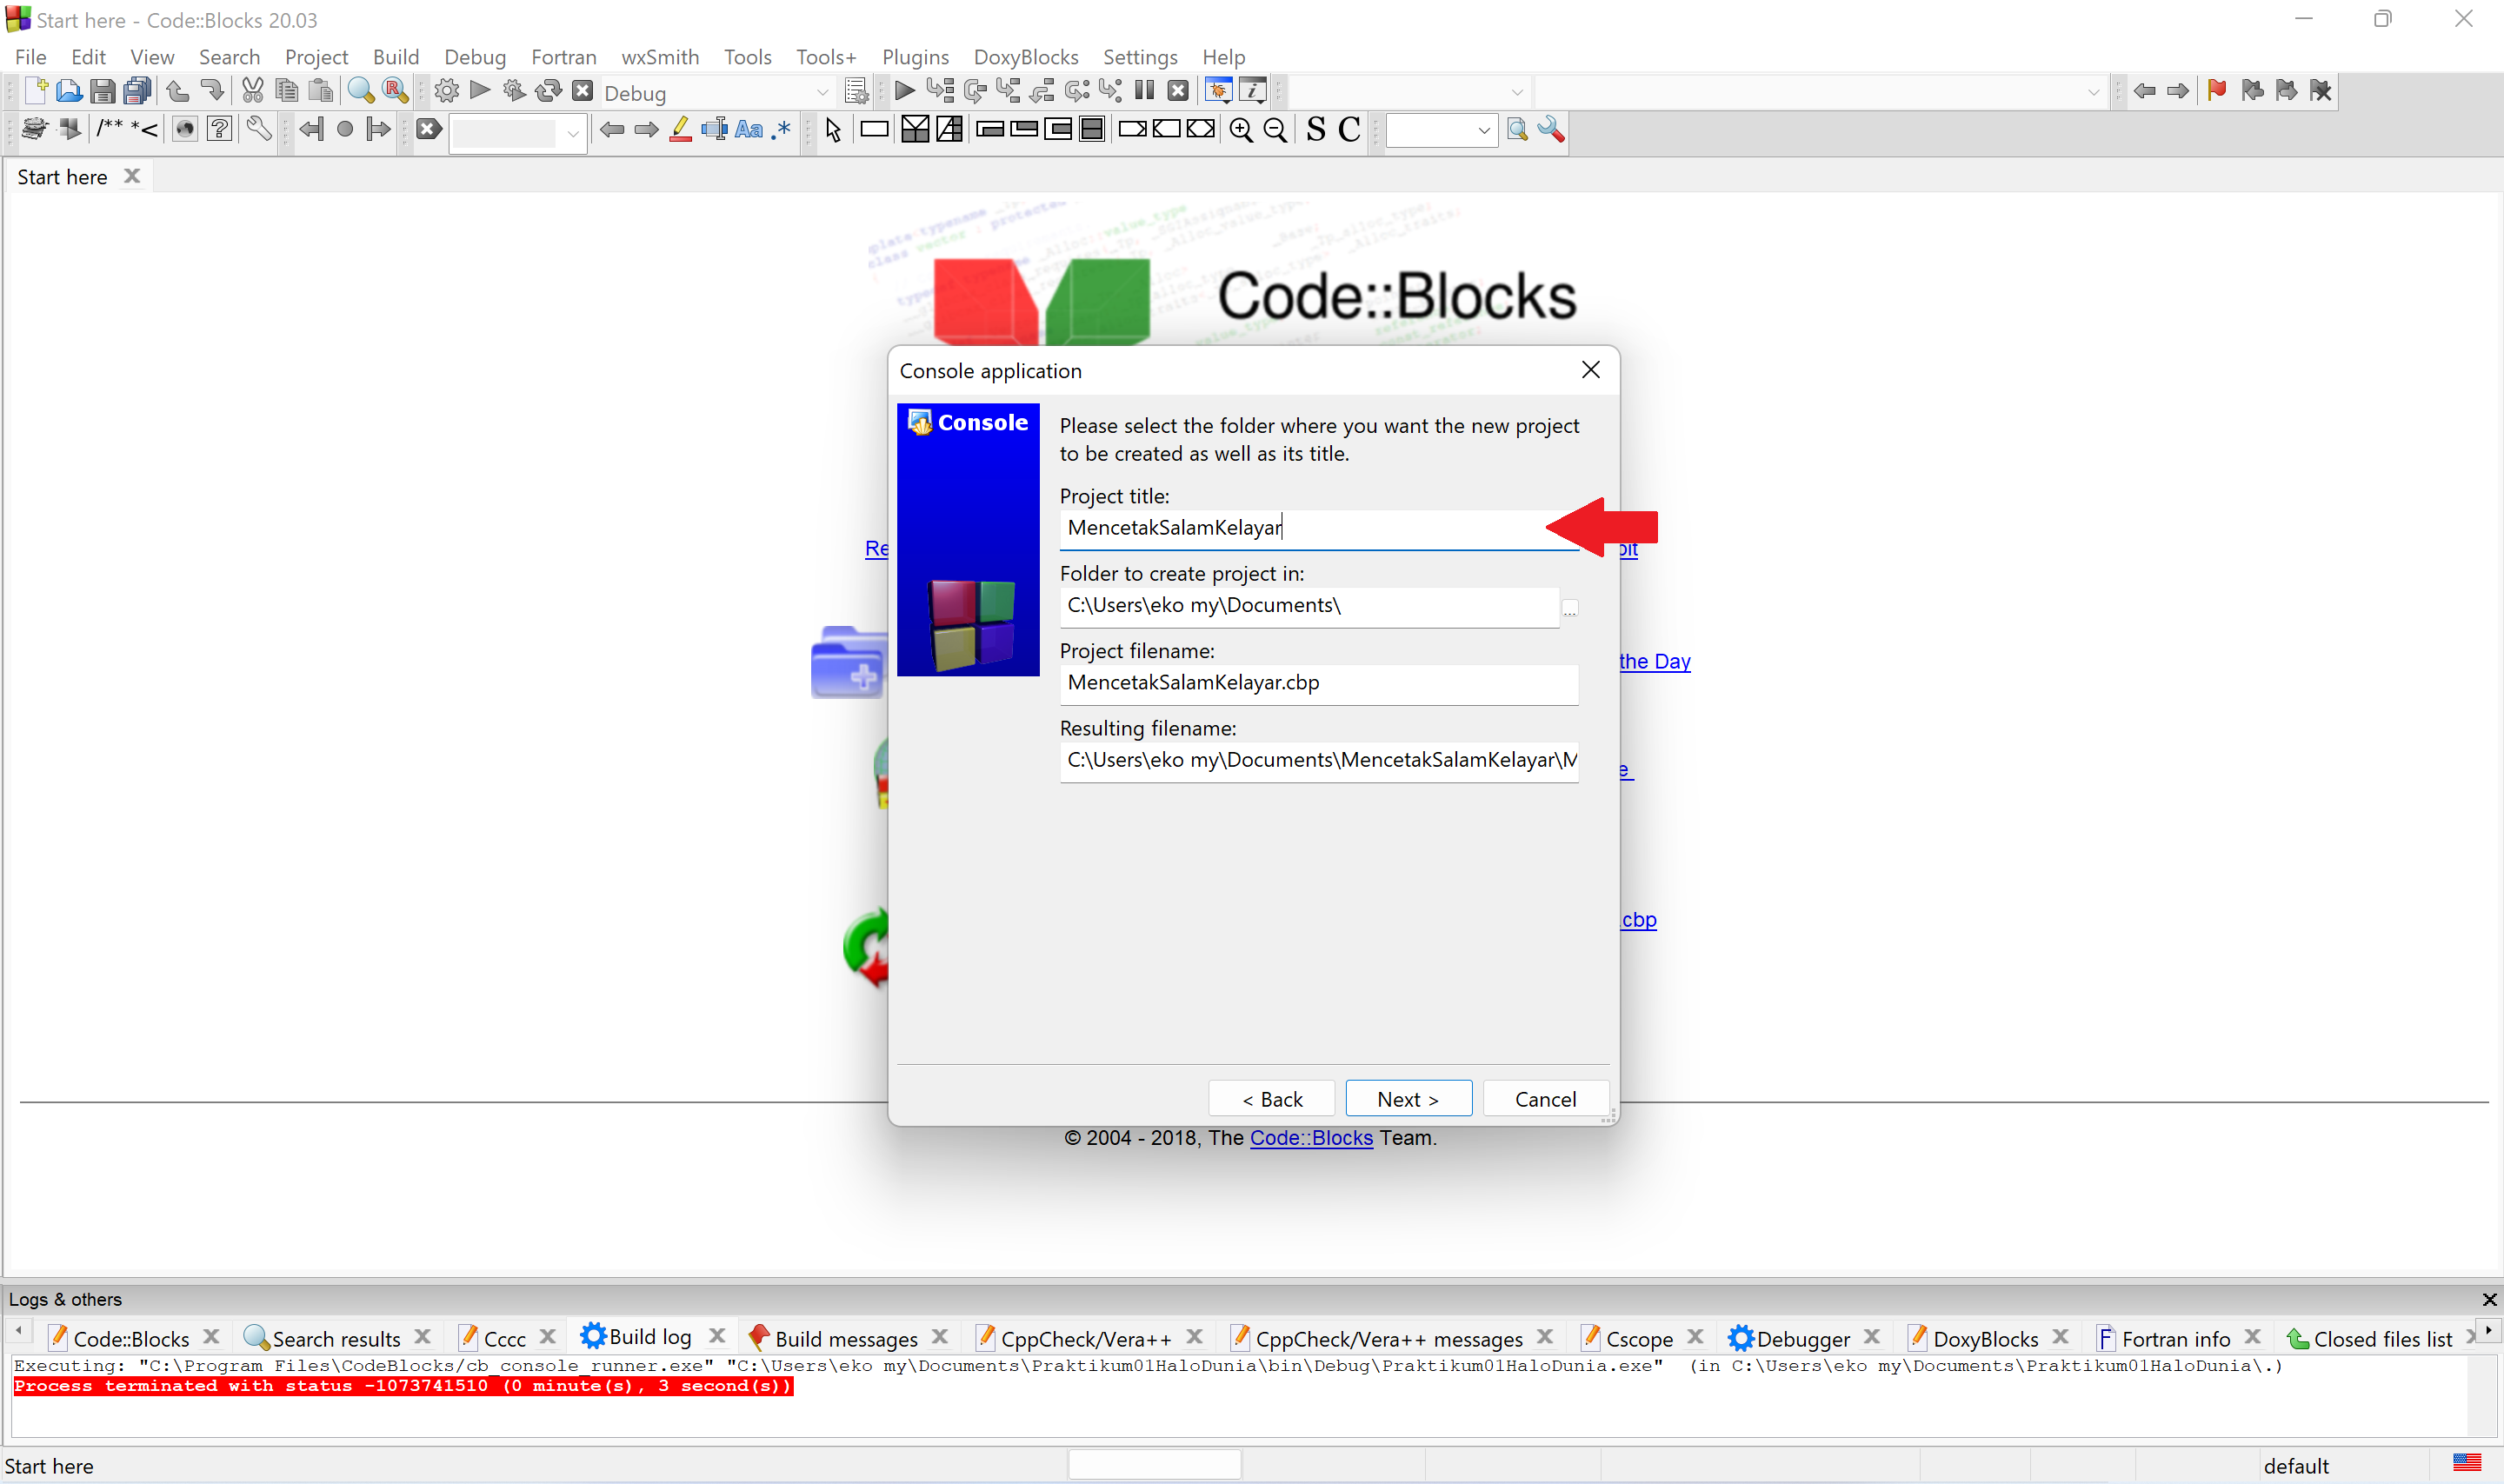
\includegraphics[width=0.7\linewidth]{P1/img/screenshot006.png}
		      \caption{}
		      \label{fig:screenshot006}
	      \end{figure}
	\item Choose the compiler (gcc), select a directory to save your project, and click save
	      \begin{figure}[H]
		      \centering
		      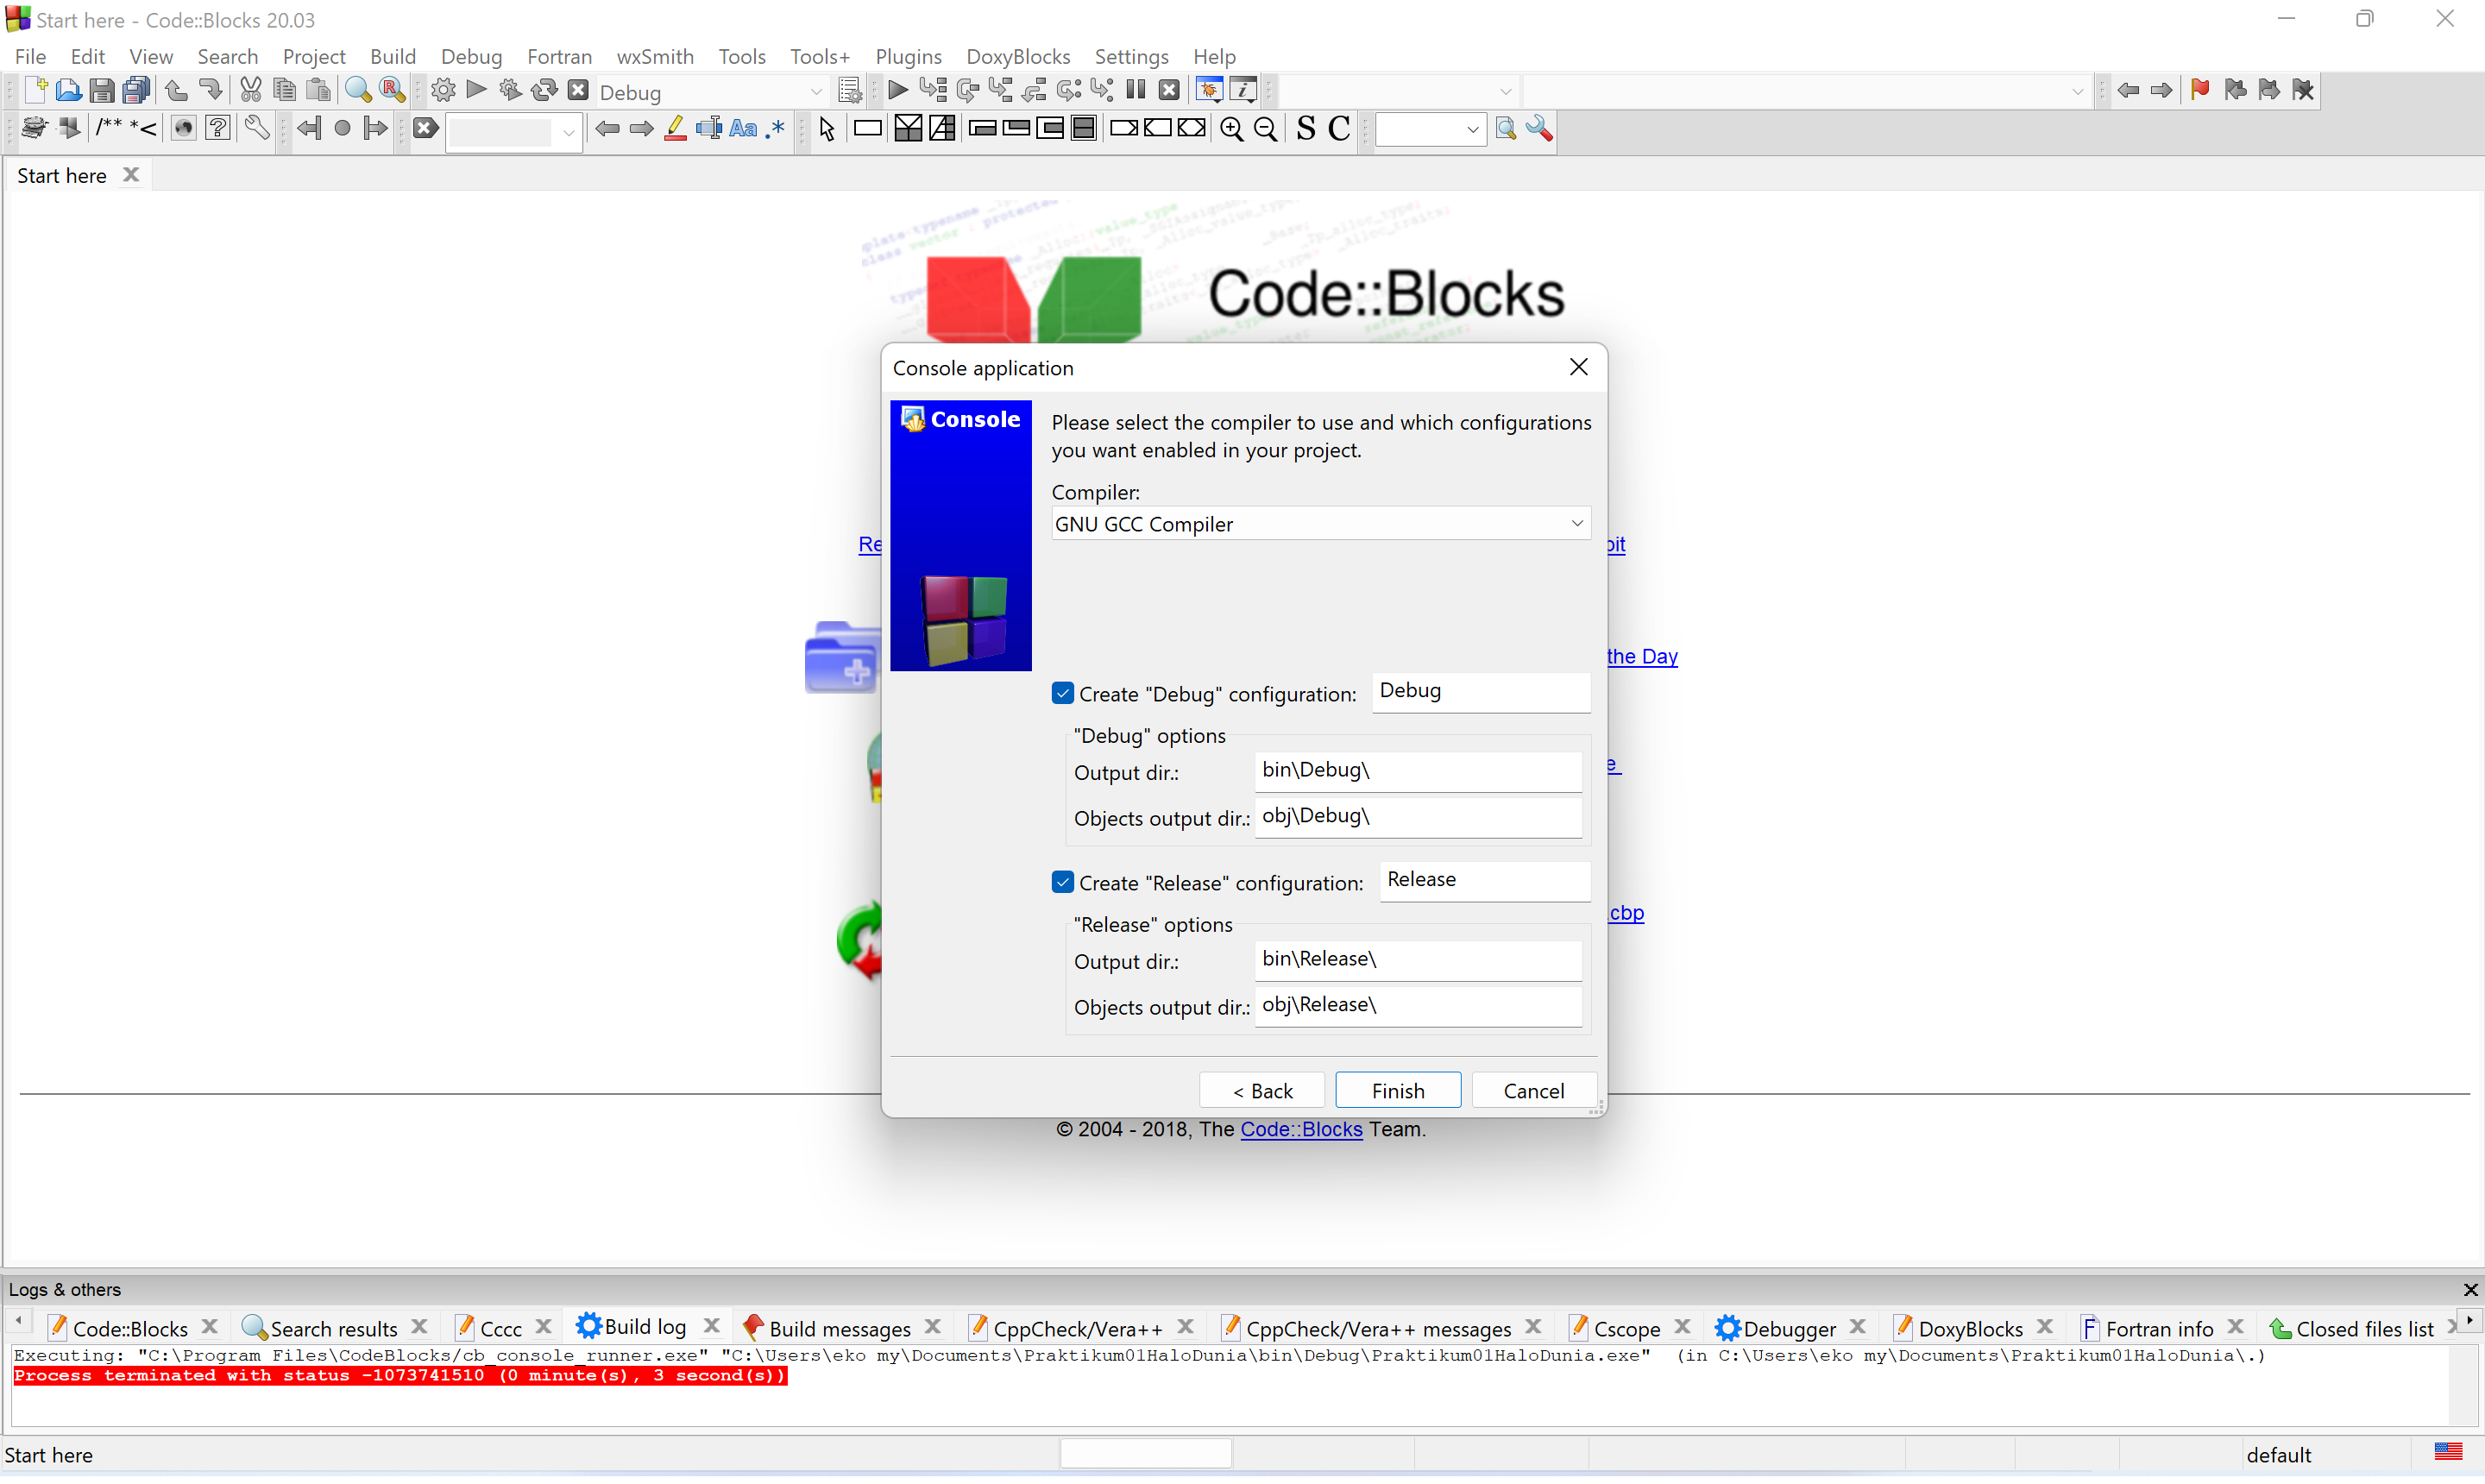
\includegraphics[width=0.7\linewidth]{P1/img/screenshot007.png}
		      \caption{}
		      \label{fig:screenshot007}
	      \end{figure}
	\item Write code as in Figure \ref{fig:screenshot008} in Code::Blocks
	      \begin{figure}[H]
		      \centering
		      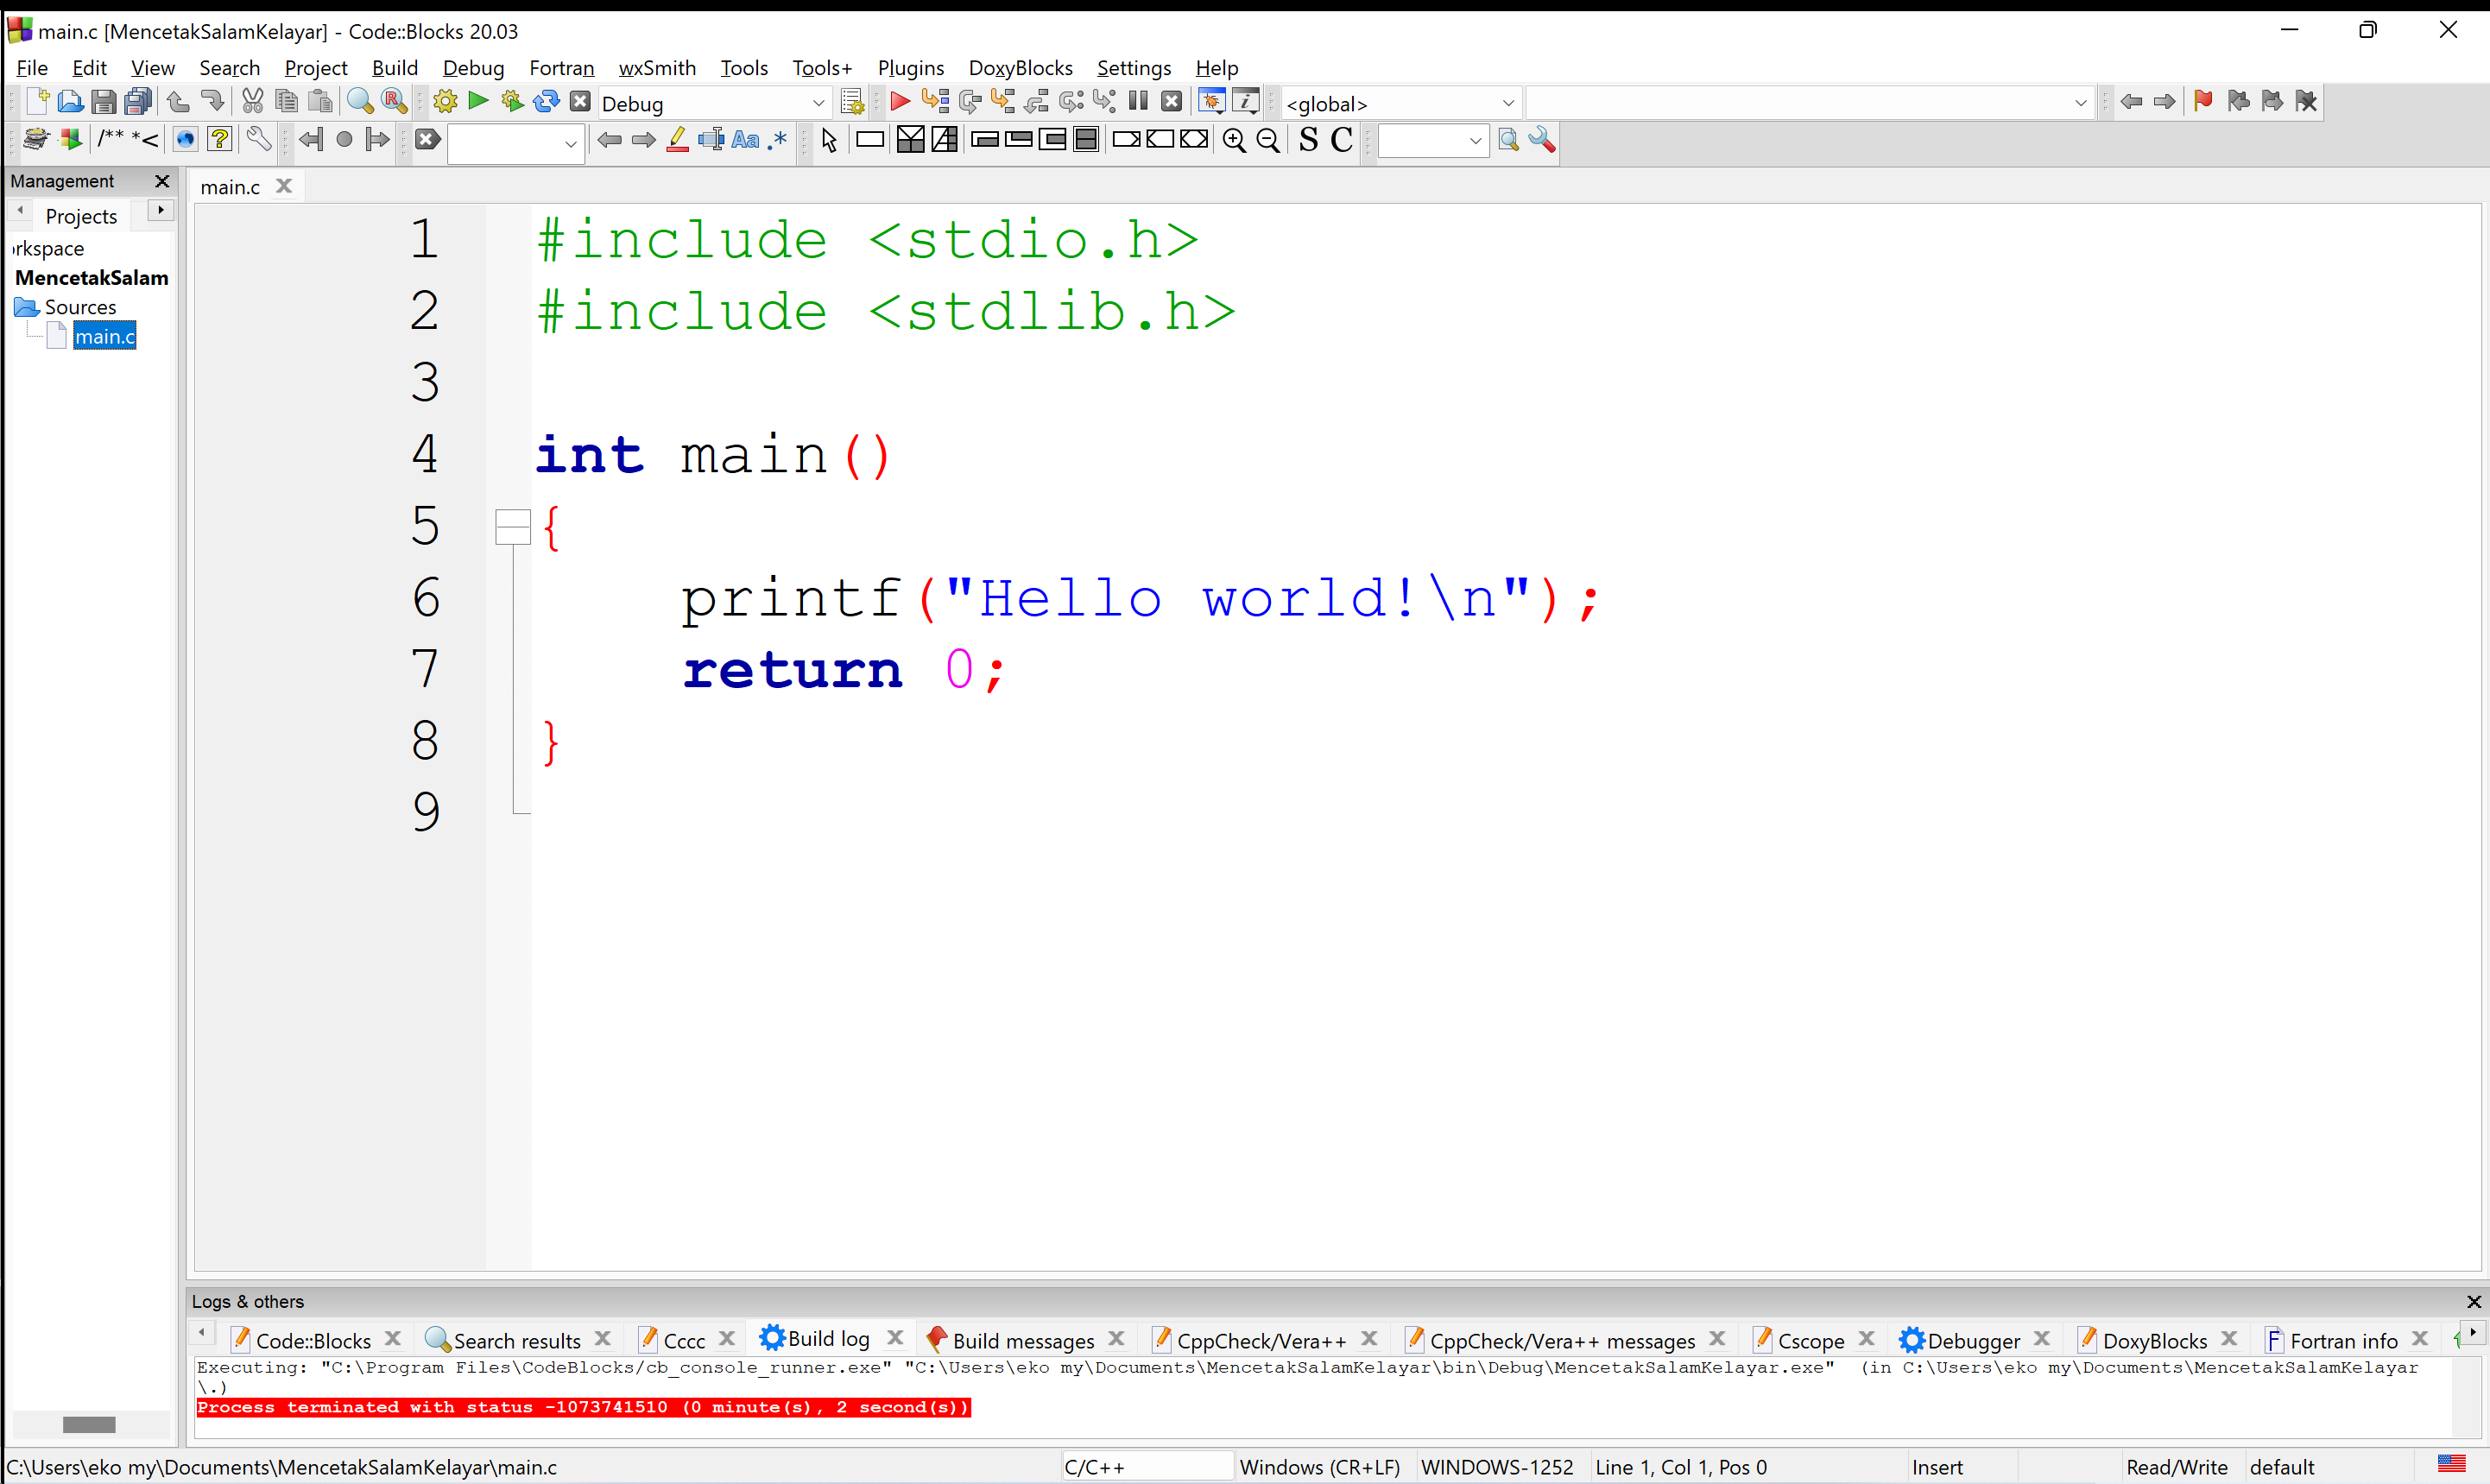
\includegraphics[width=0.7\linewidth]{P1/img/screenshot008.png}
		      \caption{}
		      \label{fig:screenshot008}
	      \end{figure}
	\item Click Build$->$Build and Run or press F9 on your keyboard
	      \begin{figure}[H]
		      \centering
		      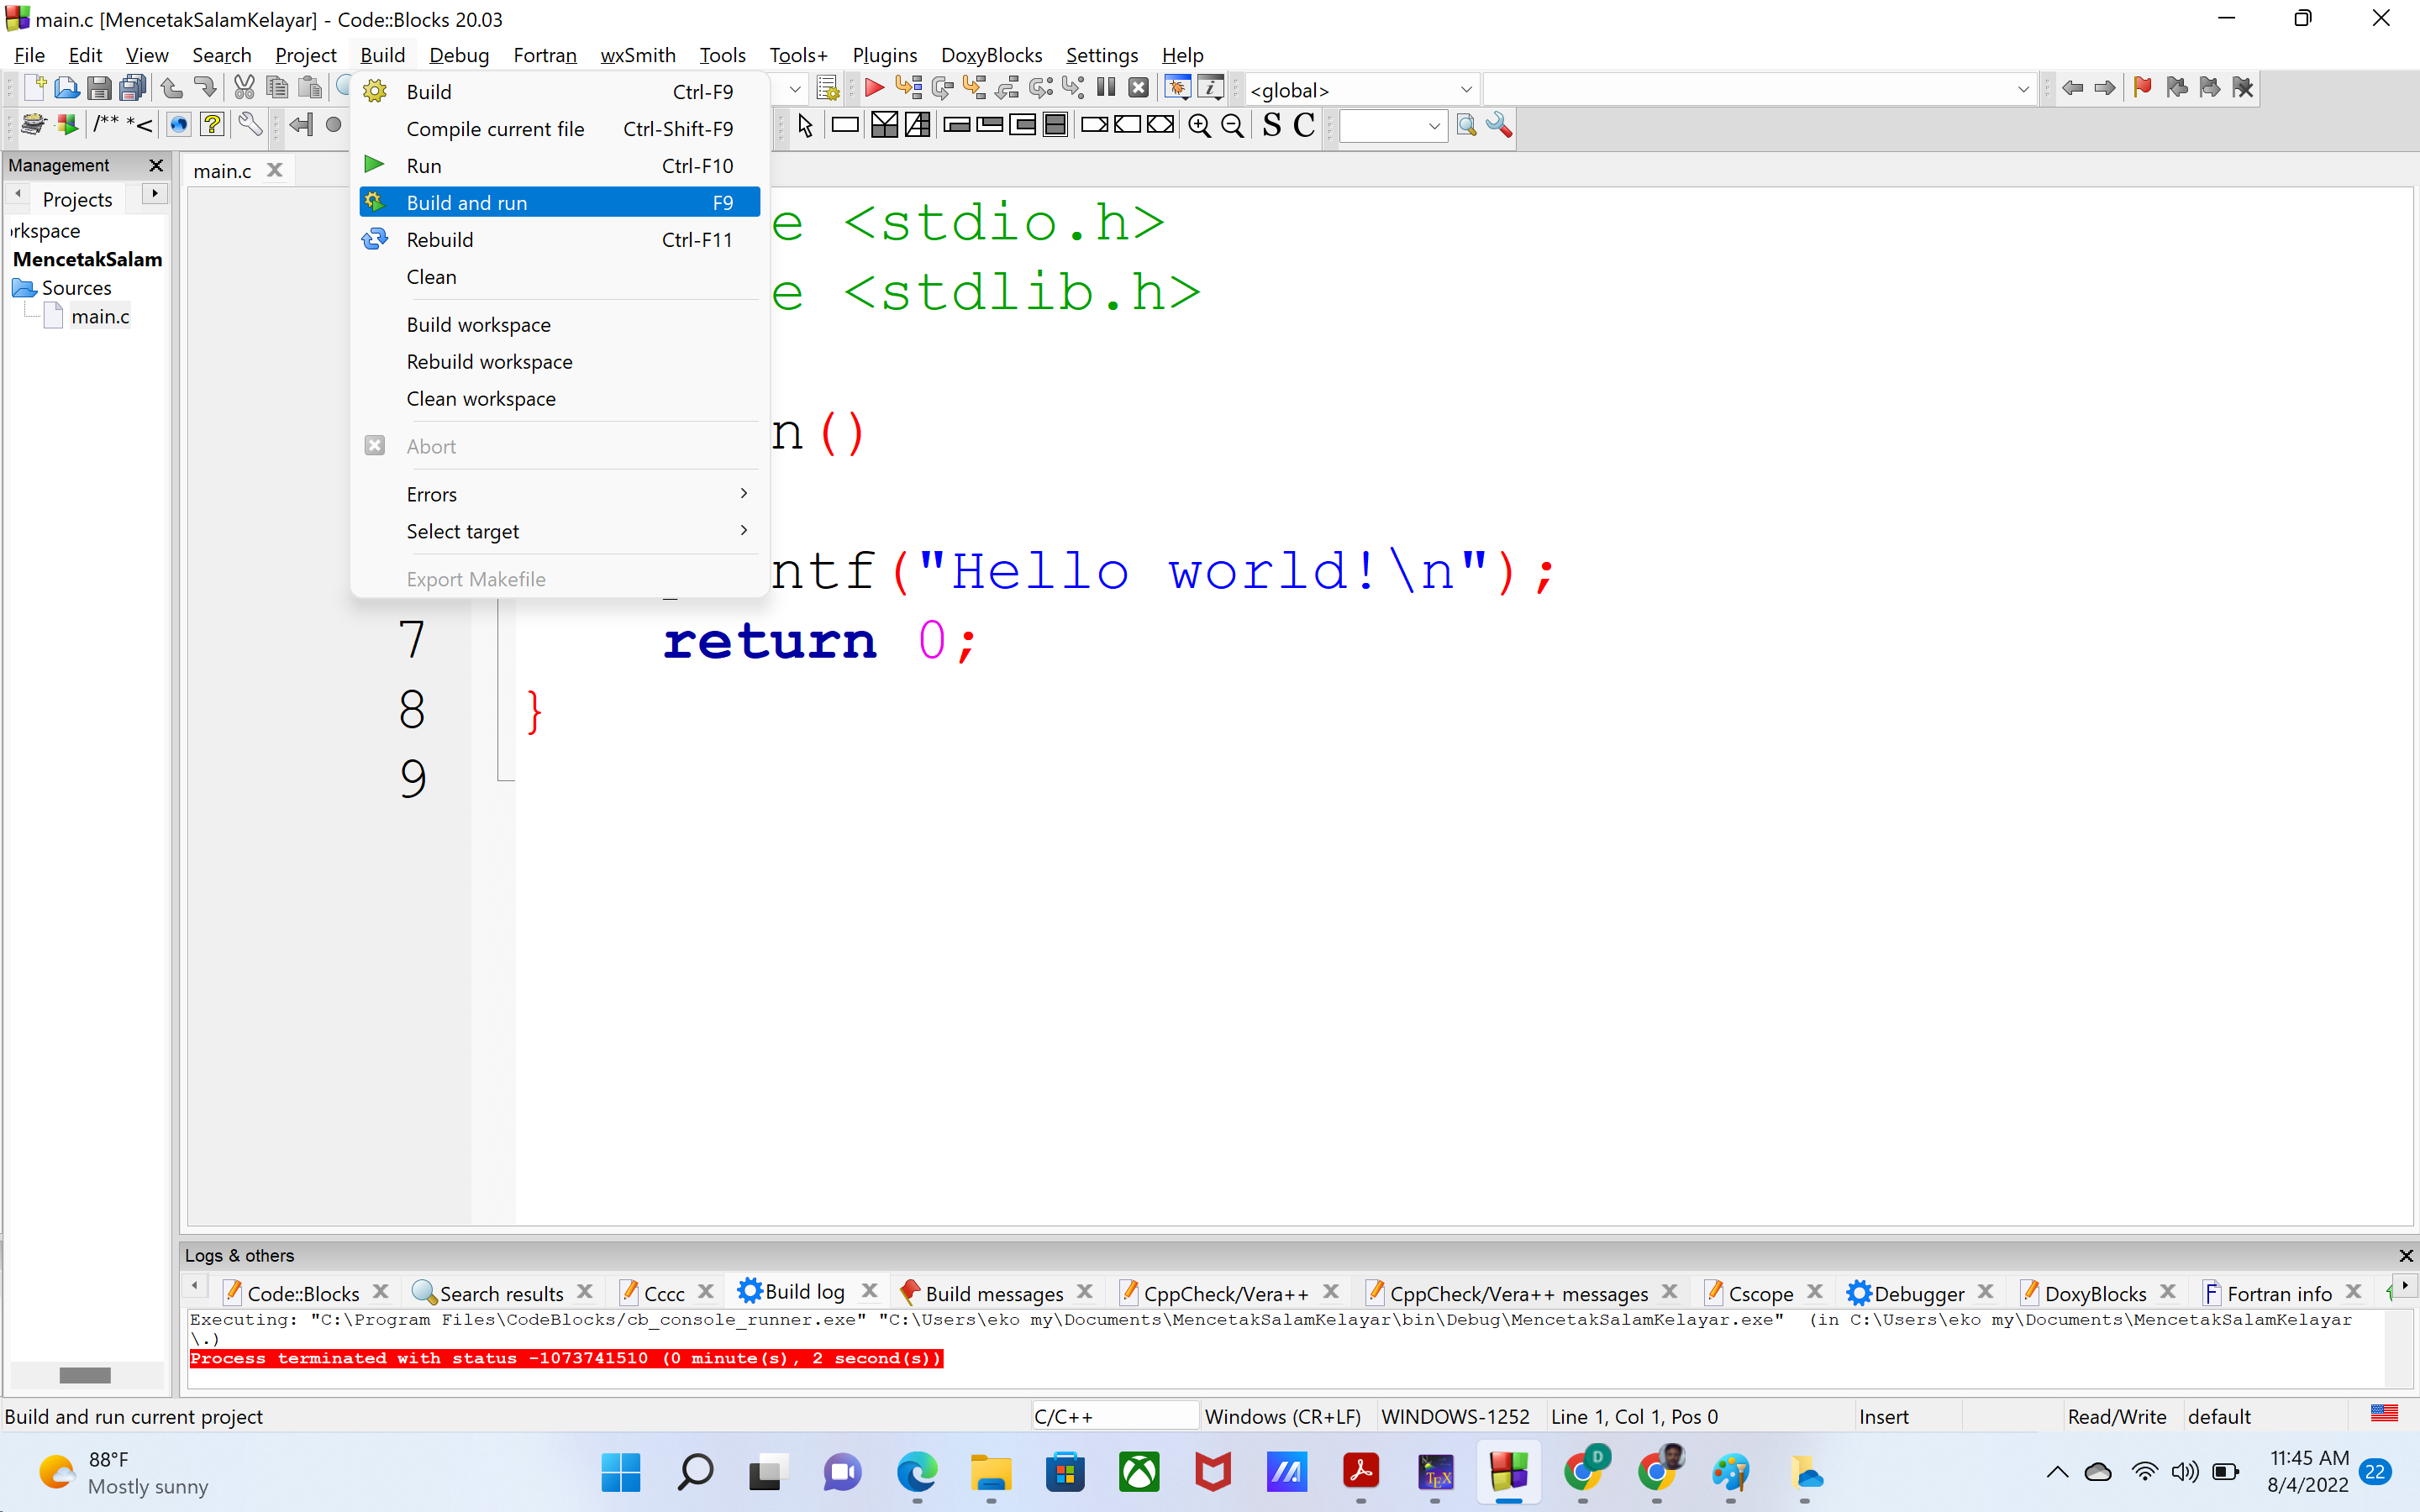
\includegraphics[width=0.7\linewidth]{P1/img/screenshot009.png}
		      \caption{}
		      \label{fig:screenshot009}
	      \end{figure}
	      % \item The program outputs can be seen on the console.
	\item The program output can be seen on the console tab
	      \begin{figure}[H]
		      \centering
		      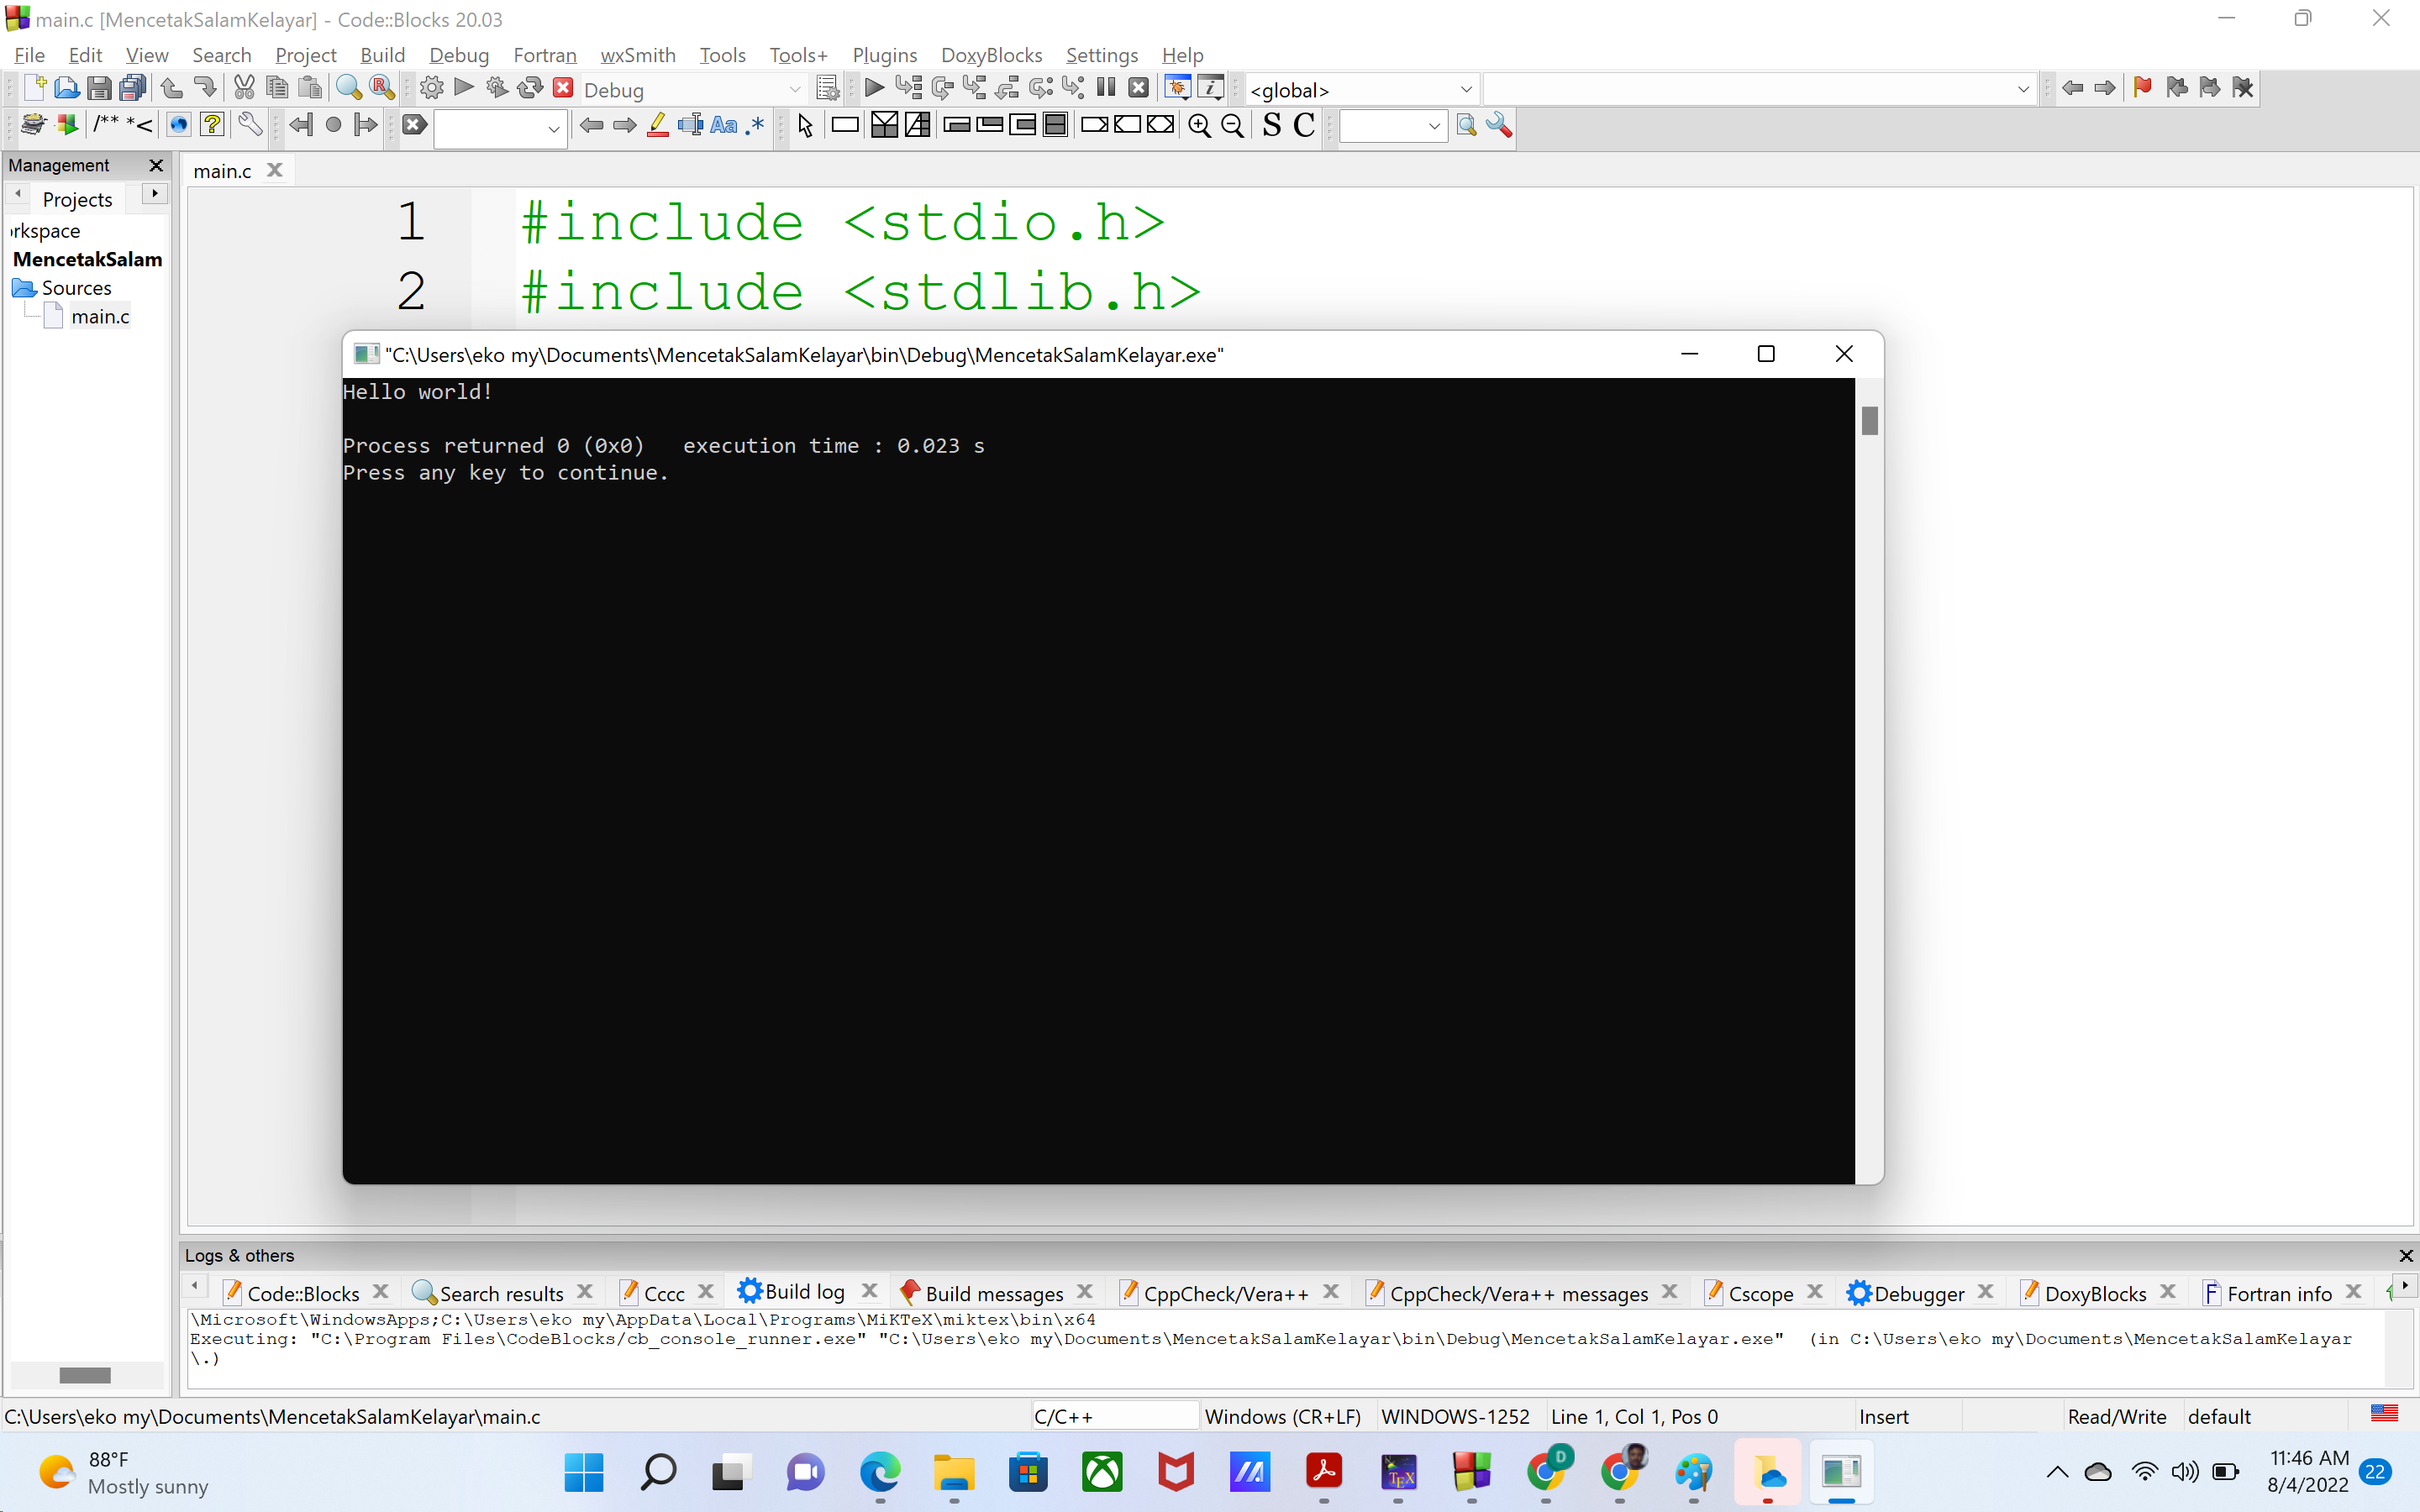
\includegraphics[width=0.7\linewidth]{P1/img/screenshot010.png}
		      \caption{}
		      \label{fig:screenshot010}
	      \end{figure}
\end{enumerate}

% \subsection{Pre-lab Assignment}
% Create a project with name HaloDunia and write the program like can be seen on figure \ref{fig:screenshot008} but change \verb|Hello World!| with \verb|Halo Dunia!|
\subsection{Pre-lab Assignment}
\begin{enumerate}
	\item Try looking for another IDE besides codeblocks, and explain the advantages and disadvantages of each IDE!
	\item What makes C different from other programming languages? explain the advantages and disadvantages!
	\item Create a project with name HaloDunia and write the program like can be seen on figure \ref{fig:screenshot008} but change \verb|Hello World!| with other words!
\end{enumerate}

%\begin{enumerate}
%	\item  Membuat program untuk menampilkan tulisan ke layar.\\
%	Langkah-langkah
%	\begin{enumerate}
%		\item Buatlah project baru dengan nama :\verb*|MencetakTextKeLayar|
%		\item Ketiklah ulang kode pada Listing \ref{lst:mencetaksalamkelayar}
%		\begin{figure}[H]
%		\begin{lstlisting}[language=c,label=lst:mencetaksalamkelayar,caption=Mencetak Teks Kelayar,captionpos=t]
%			/*Mencetak Text ke layar*/
%			
%			#include <stdio.h>
%			
%			int main()
%			{
%				//Mencetak ke layar
%				printf("Saya belajar  Pemprograman Komputer\n");
%				return 0;
%			}
%			
%		\end{lstlisting}
%	\end{figure}
%	\end{enumerate}
%\end{enumerate}
% \section{Structure of C Programming Language}
\section{Structure of C Programming Language}

\begin{lstlisting}[language=c,caption=Simple program example for C programming language,label=lst:helloworld,captionpos=t]
#include <stdio.h>

int main()
{
	//printing to screen
	printf("Halo World");
	return 0;
}
\end{lstlisting}

% Code on Listing \ref{lst:helloworld} is a simple program to print "Halo Dunia" to screen. The following is the explanation what each line of code do in the program.
Code on Listing \ref{lst:helloworld} is a simple program to print "Halo Dunia" to screen. The following is the explanation what each line of code do in the program.
\begin{itemize}\setlength\itemsep{-0.1em}
	\item [Row 1 :] \verb|#include <stdio.h>|\\ header file library for input and output functions like \verb|printf()| (the one used on line 6)
	\item[Row 2 :] Empty line.
	\item [Row 3 :] \verb|int main()|\\ The main function. The main function is the first function to be ran when the program starts.
	\item[Row 4 :] \{ \\Beginning of the \verb|main()| function code block.
		\item[Row 5 :]\verb|//printing to screen|\\ Comments. Comments are used to explain what the program is doing. Comments are ignored by the program, but helps the reader.
		\item[Row 6 :]\verb|printf("Halo Dunia");|\\ Printing "Halo Dunia" to the screen.
	\item[Row 7 :] \verb|return 0;| \\Returning the \verb|main()| function (A function ends when it returns)
	\item [Row 8 :] \}\\Closing the \verb|main()| function code block.

	      % \item [Baris 1 :] \verb|#include <stdio.h>|\\ file library header untuk fungsi input dan output seperti \verb|printf()| (contoh digunakan di baris 6)
	      % \item[Baris 2 :] Baris kosong. 
	      % \item [Baris 3 :] \verb|int main()|\\ Fungsi main. Fungsi utama adalah fungsi pertama yang akan dijalnkan ketika program dimulai.
	      % \item[Baris 4 :] \{ \\Permulaan dari \verb|main()| fungsi code block.
	      % \item[Baris 5 :]\verb|//printing to screen|\\ Komen. Komen digunakan untuk menjelaskan program. Komen akan diabaikan oleh program, tetapi membantu pembaca.
	      % \item[Baris 6 :]\verb|printf("Halo Dunia");|\\ Print/mencetak "Halo Dunia" ke layar.
	      % \item[Baris 7 :] \verb|return 0;| \\Mengembalikan \verb|main()| fungsi (sebuah fungsi berakhir ketika dikembalikan/return)
	      % \item [Baris 8 :] \}\\Menutup \verb|main()| fungsi code block.

\end{itemize}
% \subsection{Pre-lab Assignment}
% Try to swap line 6 and line 7 in Listing \ref{lst:helloworld}. What happened?\\
% What if \verb|return 0;| replaced with \verb|return 1;|?
\subsection{Pre-lab Assignment}
\begin{enumerate}
	\item Try to swap line 6 and line 7 in Listing \ref{lst:helloworld}.Explain what happened?
	\item What if \verb|return 0;| replaced with \verb|return 1;|?
	\item What happens if \verb|return 0;| is deleted?
\end{enumerate}


\section{Data Types and Variable}
\subsection{Data Types}
In C programming language, there are several data types to represent integer, real number, characters, string, and etc.
% In C programming language, there are several data types to represent integer, real number, characters, string, and etc.
\begin{center}

	\captionof{table}{Some data types in C programming language \label{tab:tipedata}}
	\begin{tabular}{|l|l|l|}
		\hline
		\textbf{Data Types}            & \textbf{Size} & \textbf{Range Value}            \\ \hline
		Int (or signed int)            & 2 bytes       & -32,768 to 32,767               \\ \hline
		unsigned int                   & 2 bytes       & 0 to 65,535                     \\ \hline
		Short int(or signed short int) & 2 bytes       & -32,768 to 32,767               \\ \hline
		Long(or singed short int)      & 4 bytes       & -2,147,483,648 to 2,147,483,647 \\ \hline
		unsigned long                  & 4 bytes       & 0 to 4,294,967,295              \\ \hline
		float                          & 4 bytes       & 1.2E-38 to 3.4E+38              \\ \hline
		double                         & 8 bytes       & 2.3E-308 to 1.7E+308            \\ \hline
		Long double                    & 10 bytes      & 3.4E-4932 to 1.1E+4932          \\ \hline
		char(or signed char)           & 1 byte        & -128 to 127                     \\ \hline
		unsigned char                  & 1 byte        & 0 to 255                        \\ \hline

		%     \captionof{table}{Beberapa tipe data di C \label{tab:tipedata}}
		% 	% \begin{tabular}{|l|l|l|}
		% 	% 	\hline
		% 	% 	Data Types & Size         & Description                                         \\ \hline
		% 	% 	int       & 2 or 4 bytes & saves integers                        \\ \hline
		% 	% 	float     & 4 bytes      & saves real numbers to 8 digit behind decimal point. \\ \hline
		% 	% 	double    & 8 bytes      & saves real numbers to 15 digits behind decimal point. \\ \hline
		% 	% 	char      & 1 byte       & saves a character                     \\ \hline
		% 	% \end{tabular}
		% 	\begin{tabular}{|l|l|l|}
		% 		\hline
		% 		Tipe Data & Ukuran       & Deskripsi                                         \\ \hline
		% 		int       & 2 atau 4 bytes & menyimpan integers.                        \\ \hline
		% 		float     & 4 bytes      & menyimpan bilangan real (8 digit dibelakang desimal). \\ \hline
		% 		double    & 8 bytes      & menimpan bilangan real (15 digit dibelakang desimal). \\ \hline
		% 		char      & 1 byte       & menyimpan sebuah karakter.                     \\ \hline
	\end{tabular}
\end{center}
% Untuk menampilkan data pada layar, setiap tipe data memiliki format specifier yang dapat digunakan pada formatted string. Berikut adalah format specifier untuk beberapa tipe data.
To show the data on screen, every data type has a format specifier that can be used on formatted string. The following is the format specifier for several data types.
\begin{center}
	\captionof{table}{Format Specifier \label{tab:formatspecifier}}
	\begin{tabular}{|l|l|}
		\hline
		\textbf{Format Specifier} & \textbf{Data Types} \\ \hline
		\%d or \%i                & int                 \\ \hline
		\%f                       & float               \\ \hline
		\%lf                      & double              \\ \hline
		\%c                       & char                \\ \hline
		\%s                       & string              \\ \hline
	\end{tabular}
\end{center}
% Masih ada lebih banyak tipe data dari pada yang dituliskan pada Tabel \ref{tab:tipedata}. Tipe-tipe data ini dan spesifikasinya bisa ditemukan dengan mudah di internet.
There are still more data types that what was written on Table \ref{tab:tipedata}. These data types and its specification can be found easily on the internet.

\subsubsection{Modifier}
In general, a modifier is a word, phrase, or clause that modifies or describes a noun or verb in a sentence. Meanwhile, in programming languages, a modifier is a keyword used to alter the behavior or characteristics of an element in a program, such as variables, functions, or classes. We use modifiers to change the range of basic data types to fit programming needs. There are four modifiers, namely:
\begin{enumerate}
	\item signed \\
	      \verb|int value = -10;| (Can store integer type variables for negative and positive values)
	\item unsigned \\
	      \verb|unsigned int count = 100;|  (Can stroe integer type variables for positive value only)
	\item long \\
	      \verb|long population = 7500000000;| (Using the long data type to store values larger than the int data type.)
	\item short \\
	      \verb|short temperature = 20;| (Using the short data type to save memory when we know that the values to be stored will be relatively small.)
\end{enumerate}


\subsection{Variable}
Variables are places to store data. Declaring a variable can be done in the following ways
\begin{lstlisting}[language=c,caption=C variable declaration,label=lst:deklarasivariabel,captionpos=t]
DataType VariableName;
\end{lstlisting}
\subsubsection{Aithmetic and Assignment Operator }
Operators are symbols that represent operations to be performed on one or more operands.
Arithmetic Operators can be used to perform arithmetic operations such as addition, subtraction, etc.
The Assignment Operator can be used to perform an operation on a variable and change the value of the variable according to the results of the operation.
\begin{center}
	\captionof{table}{Arithmetic operator in C programming language\label{tab:operatoraritmatika}}
	\begin{tabular}{|c|l|c|}
		\hline

		\multicolumn{1}{|l|}{\textbf{Operator}} & \textbf{Name}  & \multicolumn{1}{l|}{\textbf{Example}} \\ \hline
		+                                       & Addition       & \verb|x + y |                         \\ \hline
		-                                       & Subtraction    & \verb|x = y|                          \\ \hline
		*                                       & Multiplication & \verb|x * y|                          \\ \hline
		/                                       & Distribution   & \verb|x/y|                            \\ \hline
		\%                                      & Modulo         & \verb|x % y|                          \\ \hline
	\end{tabular}
\end{center}

% Tabel di bawah menunjukkan beberapa operator penugasan.
\begin{center}
	\captionof{table}{Assignment operator \label{tab:operatorpenugasan}}
	\begin{tabular}{|c|c|c|}
		\hline
		\multicolumn{1}{|l|}{\textbf{Operator}} & \multicolumn{1}{l|}{\textbf{Example}}      & \multicolumn{1}{l|}{\textbf{Similiar meaning}} \\ \hline
		=                              & x = 5                             & x = 5                                 \\ \hline
		+=                             & x += 3                            & x = x + 3                             \\ \hline
		-=                             & x -= 3                            & x = x - 3                             \\ \hline
		*=                             & x *= 3                            & x = x * 3                             \\ \hline
		/=                             & x /= 3                            & x = x / 3                             \\ \hline
		\%=                            & x \%= 3                           & x = x \% 3                            \\ \hline
		\&=                            & x \&= 3                           & x = x \& 3                            \\ \hline
		|=                             & x |= 3                            & x = x | 3                             \\ \hline
		\textasciicircum{}=            & x \textasciicircum{}= 3           & x = x \textasciicircum 3              \\ \hline
		\textgreater{}\textgreater{}=  & x \textgreater{}\textgreater{}= 3 & x = x \textgreater{}\textgreater 3    \\ \hline
		\textless{}\textless{}=        & x \textless{}\textless{}= 3       & x = x \textless{}\textless 3          \\ \hline
	\end{tabular}
\end{center}
There are also 'abbreviations' for some assignment operators such as \verb*|x+=1| and \verb*|x-=1|, which \verb*|++| and \verb*|--|.
\begin{verbatim}
    x++;
    x--;
    ++x;
    --x;
\end{verbatim}

\subsubsection{Operator Bitwise}
Bitwise operators are special operators used to handle logical operations on binary numbers in bit form. Binary numbers themselves are a type of number consisting of only two digits, which are 0 and 1. If the original value used is not in binary, it will be automatically converted by the C compiler into a binary number. For example, 7 in decimal equals 0111 in binary
\\
\begin{center}
	\captionof{table}{Bitwise operator\label{tab:operatorbitwise}}
	\begin{tabular}{|c|c|c|c|c|c|}
		\hline
		\multicolumn{1}{|l|}{\textbf{Operator}} & \multicolumn{1}{|l|}{\textbf{Name}} & \multicolumn{1}{|l|}{\textbf{Example}}   & \multicolumn{1}{|l|}{\textbf{Binary}}      & \multicolumn{1}{|l|}{\textbf{Result (binary)}} & \multicolumn{1}{|l|}{\textbf{Result (decimal)}} \\ \hline
		\&                             & AND                        & 10 \& 12                        & 1010 \& 1100                      & 1000                                  & 8                                      \\ \hline
		|                              & OR                         & 10 | 12                         & 1010 | 1100                       & 1110                                  & 14                                     \\ \hline
		\textasciicircum{}             & XOR                        & 10 \textasciicircum 12          & 1010 \textasciicircum 1100        & 0110                                  & 6                                      \\ \hline
		$\sim$                         & NOT                        & $\sim$10                        & $\sim$1010                        & 0101                                  & -11 (two complement)                   \\ \hline
		\textless{}\textless{}         & Left shift                 & 10 \textless{}\textless 1       & 1010 \textless{}\textless 1       & 10100                                 & 20                                     \\ \hline
		\textgreater{}\textgreater{}   & Right shift                & 10 \textgreater{}\textgreater 1 & 1010 \textgreater{}\textgreater 1 & 101                                   & 5                                      \\ \hline
	\end{tabular}
\end{center}

\begin{center}
	\colorbox{pink}{\parbox{0.8\linewidth}{\textbf{Notes:} There are several operators in the C language. Please study them by seeking references independently}}
\end{center}

\subsection{Pre-lab Assignment}
\begin{lstlisting}[language=c,caption=Using assignment operator in a const variable,label=lst:constassignment,captionpos=t]
#include <stdio.h>
int main()
{

	//variable declaration
    const int x=0;
    x=1;
		printf(x);
		return 0;
}
\end{lstlisting}

\begin{enumerate}
	\item Try to compile the program in Listing \ref{lst:constassignment}, what happened?
	% Coba jalankan program di Listing \ref{lst:constassignment}, apa yang terjadi?
	\item What must be done so that the output of Listing \ref{lst:constassignment} is 1 ?

\end{enumerate}
\begin{lstlisting}[language=c,caption=Using format specifier,label=lst:formspec,captionpos=t]
#include <stdio.h>
int main(){
    float a = 3.14;
    printf("%d", a);
}
\end{lstlisting}
\begin{enumerate}
	\setcounter{enumi}{2}
	%\item Coba jalankan program  di Listing \ref{lst:formspec}, apa yang terjadi? Mengapa hal itu terjadi?
	\item Try to compile the program in Listing \ref{lst:formspec}, what happened?
	%\item Apa yang harus dilakukan agar program pada Listing \ref{lst:formspec} bernilai 6.9 ?
	\item What must be done so that the program in Listing \ref{lst:formspec} has a score of 3.14?
\end{enumerate}

\section{Input and Output}

\subsection{printf()}
\verb*|printf| is a function in C that is used to print formatted string.  You can use format specifier \verb*|%| within the formatted string to outputs your variables.
% is a function in C that is used to print formatted string.
% You can use format specifier within the formatted string to outputs your variables.

\begin{verbatim}
	printf(const char *format,v1,v2,..,vn)
\end{verbatim}

% Format specifier untuk beberapa tipe data dapat dilihat pada Tabel \ref{tab:formatspecifier}
The format specifier for each data types can be seen on Table \ref{tab:formatspecifier}


\begin{description}
	\item[Contoh \thesubsection.1]  Printing text to the screen.
		\begin{lstlisting}[language=c,caption = Print text "C Programming" Ke layar,captionpos=t]
		#include <stdio.h>    
		int main()
		{ 
			// Printing text inside the " symbol
			printf("C Programming");
			return 0;
		}
	\end{lstlisting}
		\begin{itemize}
			% \item Seluruh program C harus berisi fungsi main() tempat program memulai menjalankan kode. 
			\item All C program must have main() function where the program needs to run the code.
			      % \item Fungsi \verb*|printf()| adalah library untuk mengirim output yang telah diformat ke layar.  Fungsi \verb*|printf()|  mencetak string dalam tanda dua tanda petik. 
			\item \verb*|printf()| function is a function from stdio.h library. This function outputs the string inside the symbol "" to the screen.
			\item \verb*|return 0;| statement in the \verb*|main()| function tells the program to exit.
			%\item \verb*|return 0;| pernyataan di \verb*|main()| fungsi memberitahu program untuk keluar.
		\end{itemize}
	\item [Contoh \thesubsection.2] Printing integer.
	      \begin{lstlisting}[language=c,captionpos=t]
		#include <stdio.h>
		int main()
		{
			int testInteger = 5;
			printf("Number = %d", testInteger); // <- %d format string
			return 0;
		}
	\end{lstlisting}


	      % Pada contoh ini digunakan format specifier \verb*|%d| untuk mencetak tipe data \verb*|int|. \verb*|%d| pada tex akan digantikan oleh isi dari \verb*|testInteger|. 
	      The code above uses the format specifier \verb*|%d| to prints \verb*|int| data type. The \verb*|%d| part of the string will be replaced with the value of \verb*|testInteger|.

	\item[Contoh \thesubsection.3] Real number output (float atau double)
		\begin{itemize}\label{eq:LuasSegitiga}
			\item \verb|Base|  : using \verb|float| data type.
			\item \verb|Height|: using \verb|float| data type.
			\item \verb|Area|  : using \verb|float| data type.
			      \begin{equation}
				      Area = \frac{1}{2} \times Base \times Height
			      \end{equation}
		\end{itemize}
		\begin{lstlisting}[language=c,captionpos=t]
		#include <stdio.h>
		
		int main()
		{
			// variable declaration
			float Base;
			float Height;
			float Area;
			// value initialization
			Base = 10;
			Height = 5;
			// calculating area
			Area = 0.5*Base*Height;
			// printing the text to screen
			printf("Area = %f",Area);
			return 0;
		}
		
	\end{lstlisting}

		explanation
		\begin{description}
			\item[Row 6-8]  \verb|Base|, \verb|Height| and \verb|Area| are \verb|float|data type which use to store triangle area data.
			\item[Row 10 dan 11] Value initialization to \verb|Base|=10 and \verb|Height|=5
			\item[Row 13] Calculating triangle area according to  the equation \ref{eq:LuasSegitiga}
			\item[Row 15] Printing \verb|Area| to the screen using \verb|printf| command.
		\end{description}
\end{description}

.\subsection{scanf}
Function \verb*|scanf(const char *format, ...)| reads input according to the format string.
% \verb*|scanf(const char *format, ...)| reads input according to the format string.

\begin{enumerate}
	\item Syntax
	      \begin{verbatim} scanf(const char *format, ...)
	\end{verbatim}
	\item Parameter \\
	      Format string in C consist of one or more whitespace, non-whitespace, and format specifiers.
	      % Format string pada C yang terdiri dari satu atau lebih yang terdiri dari \\
	      % Karakter Whitespace,Karakter Non-whitespace  dan  Format specifiers. 
	\item Return Value \\
	      % Ketika berhasil maka fungsi mengembalikan jumlah item dari argumen yang berhasil di baca.
	      The function will return the value of arguments it has sucessfully read.

\end{enumerate}

\begin{description}
	\item  [Example \thesubsection.4] Calculating triange \verb*|Base|   dan tinggi \verb*|Height| yang diinputkan dari keyboard.
	      \begin{lstlisting}[language=c]
#include <stdio.h>

int main()
{
	float Base, Height, Area;
	
	printf("Calculate triangle area\n");
	printf("\Insert Base= ");
	scanf("%f",&Base);
	printf("\nMasukkan Height=");
	scanf("%f",&Height);
	Area = 0.5*Base *Height;
	printf("Triangle Area = %.2f", Area);
	return 0;
}
	\end{lstlisting}
	      \begin{figure}[H]
		      \centering
		      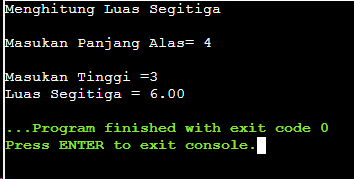
\includegraphics[width=0.5\linewidth]{P1/img/screenshot0005.png}
		      \caption{}
		      \label{fig:screenshot0005}
	      \end{figure}

	      \begin{description}
		      \item [Row 9]\verb|scanf("%f",&Area);| requesting input for triangle base
		      \item [Row 11]\verb|scanf("%f",&Height);| requesting input for triangle height
		      \item [Row 13]\verb|printf("Triangle Area = %.2f", Area);|,  \verb|.2| in \verb|%.2f| indicating that only 2 digits after the decimal point need to be printed
	      \end{description}

	\item[Example \thesubsection.5] Program to input name and email.\\
		% Pada contoh ini dipelajari bagaimana cara menginputkan string atau text dari keyboard dan mencetak kelayar. Input dari contoh program ini ada dua yang terdiri dari \verb|snama| dan \verb|sAlamatEmail|. Oleh karena text berisi banyak karakter maka masing-masing variabel dideklarasikan sebagai kumpulan karakter dengan jumlah karakter untuk sNama=20 dan sAlamatEmail=30. 
		This example shows how to input string or text from keyboard and outputs it on the screen. Input from this program consist of \verb|sName| and \verb|sEmail|. Because the text contains many characters, each variable is declared as an array of characters with the number of characters for sName=20 and sEmailAddress=30.
		\begin{figure}[H]
			\begin{lstlisting}[language=c]
		#include <stdio.h>
		
		int main () 
		{
			char sName[20], sEmail[30];
			
			printf("Enter Name: ");
			scanf("%19s", sName);
			
			printf("Enter Email: ");
			scanf("%29s", sEmail);
			
			printf("Name : %s\n", sName);
			printf("Email:%s", sEmail);
			return(0);
		}
	\end{lstlisting}
		\end{figure}
\end{description}


\subsection{Escape Sequence}
% Escape Sequence adalah urutan karakter yang digunakan untuk memformat output dan tidak ditampilkan ketika dicetak ke layar. Setiap karakter mempunyai fungsi tertentu. 
Some characters can't be written on the format string because they are used to format the outputs. So, to outputs those special characters we use escape sequences.

\begin{table}[H]
	\centering
	\captionof{table}{Escape Sequence \label{tab:escapesequence}}
	\begin{tabular}{|l|l|l|}
		\hline
		\textbf{Escape sequence}         & \textbf{Output} \\ \hline
		\textbackslash{}a                & Bell, alarm     \\ \hline
		\textbackslash{}b                & Backspace       \\ \hline
		\textbackslash{}f                & Change Page     \\ \hline
		\textbackslash{}n                & Change Row      \\ \hline
		\textbackslash{}r                & Carriage return \\ \hline
		\textbackslash{}t                & Tab Horizontal  \\ \hline
		\textbackslash{}v                & Tab Vertikal    \\ \hline
		\textbackslash{}'                & Single Quotes   \\ \hline
		\textbackslash{}"                & Double Quotes   \\ \hline
		\textbackslash{}?                & Question Mark   \\ \hline
		\textbackslash{}\textbackslash{} & Backslash       \\ \hline
	\end{tabular}
\end{table}

\begin{description}
	\item[Contoh \thesubsection.6] Change row with escape sequence \verb*|\n|.
		\begin{lstlisting}
#include <stdio.h>

int main() 
{
	printf("Halo \nI'm learning C programming language.\nand it's so fun!");
	return 0;
}
	\end{lstlisting}
		\begin{figure}[H]
			\centering
			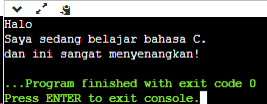
\includegraphics[width=0.5\linewidth]{P1/img/screenshot0006.png}
			\caption{}
			\label{fig:screenshot0006}
		\end{figure}

	\item[Contoh \thesubsection.7] Using escape sequence\verb*|\t| to change tab.
		\begin{lstlisting}[language=c]
#include <stdio.h>
int main(void)
{
	printf("Name \t\t: Rahmad Rahardi\n");
	printf("Address \t\t: Bendungan Hilir Jakarta\n");
	printf("Place of Birth \t: Jakarta\n");
	printf("Date of Birth \t: 30 February 2000\n");
	
	return (0);
}
\end{lstlisting}
		\begin{figure}[H]
			\centering
			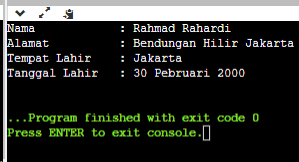
\includegraphics[width=0.5\linewidth]{P1/img/screenshot0007.png}
			\caption{}
			\label{fig:screenshot0007}
		\end{figure}
\end{description}

\subsection{Pre-lab Assignment}
\begin{enumerate}
	\item \verb|scanf("%d", &height)|, the code will ask for input to be entered in the variable \verb|height|. Explain why there is "\verb|&|" on \verb|&height|! what happens if it is simply written as \verb|height| whitout \verb|&|!
	\item Try to build a program to read input for the name and NRP and display it to the screen!
	\item Try to build a program that asks user to enter a number, then displays the squared dan cubed value of it!
\end{enumerate}

\begin{center}
	\colorbox{cyan!30}{\parbox{0.8\linewidth}{\textbf{Optional:} Learn Git and Github. You can start learning from the following resources: \\ \href{https://github.com}{GitHub - https://github.com} \\ \href{https://git-scm.com/doc}{Git -https://git-scm.com/doc}}}
\end{center}